%section{Maximizing Parallelism}

%\section{Verification and Consistency under Uncertainty}
\section{Consistency under Uncertainty}

\pbg{In this section, we describe how we use our model to efficiently synthesize update sequences that obey a set of provided invariants (\S\ref{sec:parallelism}).  We then identify a class of invariants that can be guaranteed in this manner (\S\ref{sec:seg-independence}), and present our technique to preserve consistency for broader types of invariants (\S\ref{sec:synthesis}).}

\subsection{Enforcing Correctness with \pbg{Heuristically} Maximized Parallelism}
\label{sec:parallelism}

The key goal of our system is to pbg{instill}
user-specified notions of correctness during network transitions.

Using our model to perform this task is also relatively straightforward.
We can construct a {\em buffer} of updates received from the application,
and attempt to send them out in FIFO order. Before each update is sent, we check with the
verification engine on whether there is any possibility, given the uncertainty in network state, sending it could result in an invariant violation. If so, the update remains buffered until it is safe to be sent.

There are two key problems with this approach.
The first is head-of-line blocking: it may be safe to send an update, but one before it in the queue, which isn't safe, could block it. This introduces additional delays in propagating updates
to the network.
%, which slows the convergence process and reaction to events.
Second, only one update is sent at a time, which is wasteful---if groups of updates do not conflict with each other, they could be sent in parallel.

To address this,
%\cut{As the ultimate goal of our system is t}To {\em instill} flexible and user-specified notions of correctness during network transitions,
\name provides an algorithm for synthesizing update sequences to networks that greedily {\em maximizes parallelism} while
simultaneously obeying \wxznew{the supplied}\cut{flexible consistency} properties
%\cut{.Our technical approach to maximize update parallelism subject to the \wxz{supplied} invariant(s) is
%presented in}
(Algorithm 1).%\cut{~\ref{alg:blackbox}}.  

Whenever an update $u$ is issued from the controller, 
\name intercepts it before it hits the network.
%Using the new update $u$, and all the rules that might exist in the data plane (thus including uncertain rules),
%\name finds a set of Equivalence Classes (ECs) affected by the new update.
%For each of these EC, t
Network forwarding behavior is modeled as 
an uncertainty graph ($G_{uncertain}$) as described previously.
%\cut{, which marks a subset of links as uncertain.}
Next, the black-box verification engine takes the graph and the new update as input,
and performs a computation to determine whether there is any possibility that the
update will cause the graph state to violate
%computes if the update makes the graph state any possibility of violating 
any policy internally specified within this engine.
If the verification is passed, the update $u$ is sent to the network
and also applied to the network model $Model$, but marked as uncertain.
Otherwise, the update is buffered temporarily in $Buf$.
%the black-box engine reports one or several locations where $u$ fails to satisfy the policy.
%To explain why there could be several locations, let us consider a case where a loop freedom policy is imposed.
%Whenever a violating update $u$ is captured by the black-box engine, applying this update may result a loop in the data plane.
%But the removal any link in this loop would solve the problem. 
%Thus, the correctness of issuing $u$ could be dependent on changes on any location involved in this loop.
%Then $u$ is stored at the location(s) in the dependency graph of pending updates $G_{dependency}$.
%This means, $u$ being passed to the network without violating the policy may depends on
%some updates executed on (one of several of) the locations.

%\wxzc{ to enforce consistency during network updates; 
% to maximize update efficiency.
%}
% two uses for model:
% you can use model to do veriificaiton - can find all possible bugs, and use that later to find otu why network went wrong
% or, real time response to bugs
% 
% based in info in sec 4
% doing synthesis is obvious
% here we give proposal for maximizing paralleism
% 
% why max paralleism?
% - if you just bguffer and send out in fifo order it's not efficnet, yhou get head of line blocking, and you also just do one at a time

% It is crucial to preserve key properties under network temporal uncertainty.
% By continuously verifying our uncertainty-aware network model, we are able to detect potential invariant violations, and to compute the time that the faults may occur. Such information can facilitate network operators to perform postmortem analysis, e.g., tracing back the root cause of actual invariant violations. 
% %However, in order to protect the network from errors all the time, we have to answer the question 
% %\emph{can we construct an update plan that is always compliant with specified invariant as network evolves?}
% Since most uncertainty-related bugs are transient (i.e., they may disappear before operators can react), it is important to have real-time responses to the detected potential violations.
% %In addition, errors that actually happen are only a subset of the violations captured by our model. 
% %That is, there's false positive, which makes simply blocking all problematic updates sacrifice too much.
% Also, ensuring correctness of the networks comes at the cost of disruptions to network operations (cost of time) 
% or waste of network device memory (cost of space) or both.
% Therefore, we investigate strategies to customize the update scheme according to individual invariants with the goal of achieving network correctness efficiently.

% Upon verification results, temporarily blocking problematic updates, and periodically checking
% if they are safe to pass to the network is one way to enforce correctness criteria.
% %\wxzc{
% %Just defined model. look back at figure 1. enforce. really simple.
% %totally fine way of doing things.
% %This works. 
% But it's not necessarily optimal, in the sense that there are different update orderings, and some lead to faster convergences than others. For example, it is possible to /parallelize/ updates -- send sets of updates that do not conflict with each other in parallel. Maximizing the parallelism of updates can lead to the fastest rule installation times.
% %Our goal is to achieve maximized control update parallelism 
%while preserving key properties consistently during state transitions. 
%The consistency requirement should be flexible, able to support arbitrary invariant. 
%To this end, we develop \name as a framework, which takes any arbitrary invariant(s), 
%and synthesizes an update plan to minimize update delay and preserve the given invariants all the time.

%\subsection{Algorithm}
%\label{sec:algo}
When a confirmation of $u$ from the network arrives, \name also intercepts it.
The status of $u$ in $Model$ is changed to certain, 
\wxz{either immediately (if $u$ doesn't remove any forwarding link from the graph), 
or after a delay (if it does, as described in \S\ref{sec:confirm})}.
%\mattc{I thought you said previously you don't do this right away sometimes, eg for repairs?}.
The status change of $u$ may allow some pending updates that previously failed 
the verification
%at where $u$ applied 
%\cut{now being able }
to pass it.
Each of the buffered updates 
%depending on the location of $u$ are popped out.
%that overlaps with the match field of $u$ 
is processed through the routine of processing a new update, as described above.
%\mattc{is it sufficient to just check updates that overlap in the match field?
%What about an update that affects a completely different prefix downstream, but
%the flow went through a "transformation" like NAT in between so they are
%co-dependent? And what match field are you talking about anyway?}.  

\wxzcr{In this way, \name maintains the order of updates only when it matters.
Take the example in Figure~\ref{fig:mt_example}. If the deletion of rule 1 is issued 
before the addition of rule 2 is confirmed, \name's verification engine will
capture a possible loop, and thus will buffer the deletion update. Once the confirmation of
adding rule 2 arrives, \name checks buffered updates, and finds out that
now it's safe to issue the deletion instruction.
}

\cut{
\wxz{There are several possible optimizations.  
If the desired property needs to be enforced only 
on flows that match a particular pattern, 
then upon confirmation of a previously issued update, 
only those buffered updates that match the same pattern
need to be reprocessed by the verification engine. Or, for problematic
updates, the verification engine can report the dependency relationship between
the new updates and in-flight updates.
Then, confirming an update will trigger the verification
engine to check only those buffered updates that depend on the confirmed update.
However, those optimizations require that the verification engine reveals extra information.
To make the design policy-agnostic, we stick with the
pure black-box approach, and evaluation results show that it performs well in
practice.}
} 
%One difference is if a pending update doesn't pass verification, it is put back to $G_{dependency}$,
%on a updated location.


\begin{algorithm}[t]
  \small
%\caption{\name's algorithm to maximize the parallelism for network update execution}
%\caption{\name's algorithm for synthesizing update orderings that maximize parallelism of installation}
\caption{Maximizing network update parallelism}
\bf{ScheduleIndividualUpdate}($Model, Buf, u$)
\begin{algorithmic} 
\State \bf{On issuing $u$:}
\State $G_{uncertain}$ = ExtractGraph($Model, u$)
\State $verify$ = BlackboxVerification($G_{uncertain}, u$)
\If {$verify$ == PASS }
        \State Issue $u$
        \State Update($Model, u, uncertain$)
\Else
        \State Buffer $u$ in $Buf$
\EndIf

\State
\State On confirming $u$:
\State Update($Model, u, certain$)
\State $Issue\_updates \gets \emptyset$
\For {$u_b \in Buf$}
        %\IF {$u_p$ overlaps with $u$}
                \State $G_{uncertain}$ = ExtractGraph($Model, u_b$)
                \State $verify$ = BlackboxVerification($G_{uncertain}, u_b$)
                \If {$verify$ == PASS }
                        \State $Buf$ removes $u_b$
                        \State Update($Model, u_b, uncertain$)
                        \State $Issue\_updates \gets Issue\_updates + u_b$
                \EndIf
        %\ENDIF
\EndFor
\State Issue $Issue\_updates$
\label{alg:blackbox}
\end{algorithmic}  
\end{algorithm}

\subsection{Segment Independence}
\label{sec:seg-independence}

Next, we identify consistency policies that guarantee
the existence of feasible update orders, 
and prove \name's heuristic guarantees to find one such order.
As defined in \cite{Reitblatt2012}, {\em trace properties} characterizes
the paths that packets traverse through the network.  This covers many common network properties, including reachability, access control, loop freedom, and waypointing.
%including basic reachability, access control, loop freedom, VLAN leak freedom, waypointing, \kevin{and many more}.
%Our discussion will first focus on trace properties, and then extend to other properties,
%such as congestion freedom.
\wxzcr{We start with the assumption that a network configuration 
applies to exactly one equivalence class of packets.}
A network configuration can be expressed as a set of paths that packets are allowed to take,
i.e., a forwarding graph, 
A configuration transition is equivalent to a transition from an initial forwarding graph, $G_0$,
to a final graph, $G_f$, through a series of transient graphs, $G_t$s. 
%Let us start from two specific trace properties: loop freedom and black-hole freedom.

\paragraph{Loop and black-hole freedom}

%We prove the following theorems for loop freedom~\cite{loopfree}:
%For loop freedom, 
The following theorems were proved for loop freedom~\cite{loopfree}:
First, given both $G_0$ and $G_f$ are loop-free,
during transition, it is safe (causing no loop) to update a node in a $G_t$ if that node satisfies 
one of the following two conditions: (1) in $G_t$ it is a leaf node, or all its upstream nodes
have been updated with respect to $G_f$; or (2) in $G_f$ it reaches the destination directly,
or all its downstream nodes in $G_f$ have been updated with respect to $G_f$.
Second, if there are several updatable nodes in a $G_t$, any update order among these nodes is
loop-free. Third, in any loop-free $G_t$ (including $G_0$) that is not equal to $G_f$,
there is at least one node safe to update, i.e., a loop-free update order always exists.

%. That is, there always exists a loop-free update order.

%\begin{theorem} (Updatable conditions): In a transition from an initial
%forwarding graph $G_0$ to a final forwarding graph $G_f$, a node update does not
%cause a transient loop in any transient forwarding graph $G_t$ (including $G_0$), 
%if it fulfils one of the following conditions:
%\begin{itemize}[noitemsep,topsep=0pt,leftmargin=*]
%\item In $G_t$ , the node is a leaf node or all its
%upstream nodes have been updated with respect to $G_f$.
%\item In $G_f$
%, the node reaches the destination directly, or all its downstream nodes in
%$G_f$ have already been updated with respect to $G_f$ in $G_t$ .
%\end{itemize}
%\end{theorem}
%
%\begin{theorem} (Simultaneous updates): If there are several updatable nodes in
%a $G_t$, then any update order among these nodes is
%loop free.  
%\end{theorem}
%
%\begin{theorem} (Existence of a loop-free update order): In a transition from
%$G_0$ to $G_f$, in any transient consistent forwarding graph $G_t$ that is not
%equal to $G_f$ (including $G_0$), at least one of the node is updatable. 
%Also, there is a loop-free update order.  
%\end{theorem}

%What \name aproves to update always results in a loop free graph, 
%so there exists an update order
%from that transient loop free graph to the final graph
%that \name is able to find.

%\paragraph{black-hole freedom} 

Similarly, we have the following proved for the black-hole freedom property~\cite{gcc_tr}.

  \vspace{-0.1in}
\begin{lemma} (Updatable condition):
A node update does not cause any transient black-hole,
if in $G_f$, the node reaches the destination directly, or
in $G_t$, all its downstream nodes in $G_f$ have already been updated.
\end{lemma}
  \vspace{-0.1in}

  \vspace{-0.1in}
\begin{proof} By contradiction. Let $N_0$, $N_1$,...$N_n$ be downstream
nodes of $N_a$ in $G_f$. Assume $N_0$, $N_1$,...$N_n$ 
have been updated with respect to $G_f$ in $G_t$.
After updating $N_a$ in $G_t$, $N_0$, $N_1$,...$N_n$ become $N_a$'s
downstream nodes and
%they have been updated with respect to $G_f$ according to the
%assumption. 
%After updating $N_a$, 
all nodes in the chain from $N_a$ to $N_n$ have been updated. % with respect to $G_f$. 
 $Na$'s upstream with respect to $G_t$ can still reach $N_a$, and thus reach the downstream of $N_a$.
If we assume there is a black-hole from updating $N_a$,
there exists a black-hole in the chain from $N_a$ to $N_n$.
Therefore, the black-hole will exist in 
%the final forwarding graph. However, since the final forwarding graph
$G_f$, and there is a contradiction.
\end{proof}
  \vspace{-0.1in}


  \vspace{-0.1in}
\begin{lemma} (Simultaneous updates): In
a $G_t$, any update order among updatable nodes is black-hole-free.  
\end{lemma}
  \vspace{-0.1in}

  \vspace{-0.1in}
\begin{proof} Consider a updatable node $N_a$ that all its downstream nodes in
$G_f$ have already been updated in $G_t$ (Lemma 1). 
Then updating any other updatable node does not change this
property. When a node is updatable it remains updatable even after updating
other nodes. Therefore, if there are several updatable nodes, they can be
updated in any order or simultaneously.  
\end{proof}
  \vspace{-0.1in}

  \vspace{-0.1in}
\begin{theorem} (Existence of a black-hole-free update order): 
In any black-hole-free $G_t$ that is not $G_f$ 
(including $G_0$), at least one of the nodes is updatable, i.e., there is a black-hole-free update order.
\end{theorem}
  \vspace{-0.1in}

  \vspace{-0.1in}
\begin{proof} By contradiction. 
Assume there is a transient graph $G_t$ such that
no node is updatable.  All nodes are either
updated or not updatable. As nodes with direct links to the destination are
updatable (Lemma 1), these nodes can only
be updated. Then nodes at previous hop of these nodes in $G_t$ are also updatable (Lemma 1), 
and therefore these nodes must also be updated. Continuing,
 it follows that all nodes are updated, which is a
contradiction as $G_t$ = $G_f$ . As there is always a node updatable
in a consistent $G_t$, and the updatable node can be
updated to form a new consistent $G_t$, 
%In each new transient graph, 
the number of updated nodes will increase.
Eventually, all nodes will be updated. Therefore there is a black-hole free
update order.
\end{proof}
  \vspace{-0.1in}
%
%Similarly, 
%It is obvious that updates fulfilling the condition of black-hole freedom 
%maintain the transient graph free as well.
%It can be easily proven that fulfilling the first condition of loop free update is not sufficient 
%to ensure black-hole freedom.
Any update approved by \name
results in a consistent transient graph,
\wxzcr{so \name always finds a consistent update sequence} 
%so there exists an update order from that transient graph to the final graph,
to ensure loop and black-hole freedom.
%It can be easily proven that fulfilling the first condition of loop free update is not sufficient 
%to ensure black-hole freedom. 
%Therefore, black-hole freedom is downstream dependent, whereas loop freedom is upstream 
%\textbf{or} downstream dependent, and thus weaker than black hole freedom.

\paragraph{Generalized Trace Properties}

\cut{
\begin{table}[!th]
\centering
\footnotesize
\caption{Consistency space}
\label{tab:space}
\begin{tabular}{|p{3.5cm}|p{3.8cm}|}
%\begin{tabular}{|l|c|c|}
\hline
Consistency property (Invariant) & Dependency among updates\\
\hline \hline
Eventual consistency & None \\ \hline
Memory limit & Self \\ \hline
Loop freedom & Downstream or upstream\\ \hline
black-hole freedom & Downstream \\ \hline
Waypoint traversal & ? \\ \hline
Isolation & ? \\ \hline
Middlebox chain & ? \\ \hline
Packet coherence & All downstream \\ \hline
QoS(Bandwidth limit)... &  \\ \hline
\end{tabular}
\end{table}
}

To get a uniform abstraction for trace properties, let us first visit
the basic connectivity problem: node $A$ should reach node $B$ ($A \rightarrow B$).
To make sure there is connectivity between two nodes, both black-hole and loop freedom properties need to hold.
Obviously, black-hole freedom is downstream-dependent (Theorem 2), whereas loop freedom is 
upstream- (updatable condition (1)) \textbf{or} downstream-dependent (updatable condition (2)), 
and thus weaker than black-hole freedom.
In other words, connectivity is a downstream-dependent property, 
i.e., updating from downstream to upstream is sufficient to ensure it.
%To start with, a simplest configuration:
%before and after forwarding graph are both a path.  For basic reachability
%($A\rightarrow B$), 
%In this case, downstream dependency (updating from downstream to upstream
%) is sufficient to guarantee consistency, as proved in black-hole freedom case.  
\wxzcr{Fortunately, a number of trace properties, such as 
waypointing, access control, service/middle box chaining, etc., 
can be broken down to basic connectivity problems.
A common characteristic of such properties is that
flows are required to traverse a set of waypoints.}

\cut{
\begin{itemize}[noitemsep,topsep=0pt,leftmargin=*] 
%\item Loop freedom: flow from any ingress node
%can reach a sink(drop) or an egress 
%\item black-hole freedom: flow from any
%ingress node can reach an egress 
\item Waypointing:
% (filter, FW, other types of middlebox): 
packets
% \cut{from any ingress }
should reach a waypoint $W$;
\item Isolation: packets flowing between isolated domains must encounter a filter/drop node; 
\item Middlebox chain: packets must traverse a chain of middleboxes ($A\rightarrow M1 \rightarrow M2 \rightarrow B$);
\item Combinations of the properties above: for example,
packets from $A$ must reach its destination $B$, and traverse a waypoint $W$ before reaching $B$ ($A\rightarrow W\rightarrow B$).
\end{itemize}
%Combinations of the properties above,

For properties with points on the path that must be traversed,
%(e.g., $A\rightarrow B\rightarrow C$),
we refer to these points as {\em waypoints}. 
%Suppose we want flows to traverse the waypoints in a
%particular order. %(stronger than without the order constraint). 
%For simplicity, assume single-path routing, and assume that policy is a group of paths,
%each starting from an ingress node.
Then $n$ waypoints divide both the old and new paths into $(n - 1)$ {\em segments}. 
}

  \vspace{-0.1in}
\begin{definition} {\bf Waypoints-based trace property:} A property
that enforces a group of packets traverse a set of
waypoints (including source and destination) in a particular order.
\end{definition}
  \vspace{-0.1in}

%Then $n$ waypoints divide both the old patch and new path each into $(n - 1)$ {\em segments}. 
%This type of invariants covers a large set of common \wxzc{?} network invariants,
%and thus it is the focus of our discussion. 
%Intuitively, 
%However, whether or not there exist dependencies among segments is determined by both the policy and topology. 
%Basic reachability: the nodes where new and old path cross also cut the new path into segments , and each segments can be updated independently in a way:
%first update all but the first hop of the section simultaneously, and second update the first hop, which guarantees the basic reachability requirement. 
%Covers a large set of common invariants:
%\begin{itemize}
%\item black-hole freedom
%\item Loop freedom
%\item Basic Reachability Policy: Suppose we wish to ensure that a server port should (not) be reachable from guest machine ports 
%\item isolation (think the filtering/dropping point in the middle of two isolated nodes as the waypoint of the flow between the two nodes)
%\item flows from certain sources must go through a middle box $M$
%\item flows that pass one middle box $M1$ must pass $M2$ next
%\item ...
%\end{itemize}

%\begin{definition} {\bf Path segment}:
%The path between two subsequent waypoints a flow is required to pass.
%\end{definition}

  \vspace{-0.1in}
\begin{definition} 
{\bf Segment dependency:}
Suppose a trace property enforces $n$ waypoints, 
which divide the old and the new flow path each into $(n - 1)$ segments:
$old_1, old_2, ..., old_{n - 1}$ and $new_1, new_2, ..., new_{n - 1}$.
If $new_j$ crosses $old_i$ ($i \ne j$), then the update of segment $j$ is 
{\bf dependent} on the update of segment $i$, 
i.e., segment $j$ cannot start to update until segment $i$'s update has finished,
in order to ensure the traversal of all waypoints. 
\end{definition}
  \vspace{-0.1in}

Otherwise, if segment $j$ starts to update before $i$ has finished, there might be
violations. If $j < i$, there might be a moment when the path between waypoints $j$
and $i+1$ consists only of $new_j$ and part of $old_i$, i.e., waypoints $(j+1)
... i$ are skipped. As in Figure~\ref{fig:circular}(b), $B$ may be skipped
if the $AB$ segment is updated before $BC$, and the path is temporarily $A \rightarrow 2 \rightarrow C$. 

If $j > i$, there might be a moment when the path between waypoints
$i$ and $(j+1)$ consists of $old_i, old_{i+1}, ..., new_j$, and a loop is formed.
As in Figure~\ref{fig:circular}(c), the path could temporarily be $A \rightarrow B \rightarrow 1 \rightarrow B$.

\wxzcr{If there is no dependency among segments 
(Figure~\ref{fig:circular} (a)), then each can be updated
independently simply by ensuring connectivity between the segment's endpoints.}
%, and is equivalent to a path with only two waypoints (source and destination). 
That suggests that for paths with no inter-segment dependencies, 
a property-compliant update order always exists.
Another special case is circular dependency between segments, as depicted in Figure~\ref{fig:circular}(d), 
in which no feasible update order exists.
%Examples of dependencies between segments (Figure~\ref{fig:circular}):
%\begin{itemize}[noitemsep,topsep=0pt,leftmargin=*]
%\item Case 1:no crossing, update different segments in parallel, as long as each segment
%updating follows downstream dependency
%\item Case 2: new BC segment crosses old AB segment, so BC depends on AB
%\item Case 3: new AB segment crosses old BC segment, so AB depends on BC
%\item Case 4: new BC segment crosses old AB segment, so BC depends on AB. new AB
%segment crosses old BC segment, so AB depends on BC. Results in circular dependency ==>
%no feasible order exist ==> use higher consistency level tool (e.g., CU)
%%\item Case 5: More than two segments $A\rightarrow B\rightarrow C\rightarrow D$
%%new CD segment crosses old AB segment, so CD depends on AB.
%%AB and BC can be updated in parallel, but CD has to wait for AB update finish.
%\end{itemize}

\begin{figure*}[!th]
  \vspace{-0.1in}
  \centering
  \subfigure[No segment crossing, update different segments in parallel, as long as each segment's updating follows downstream dependency]{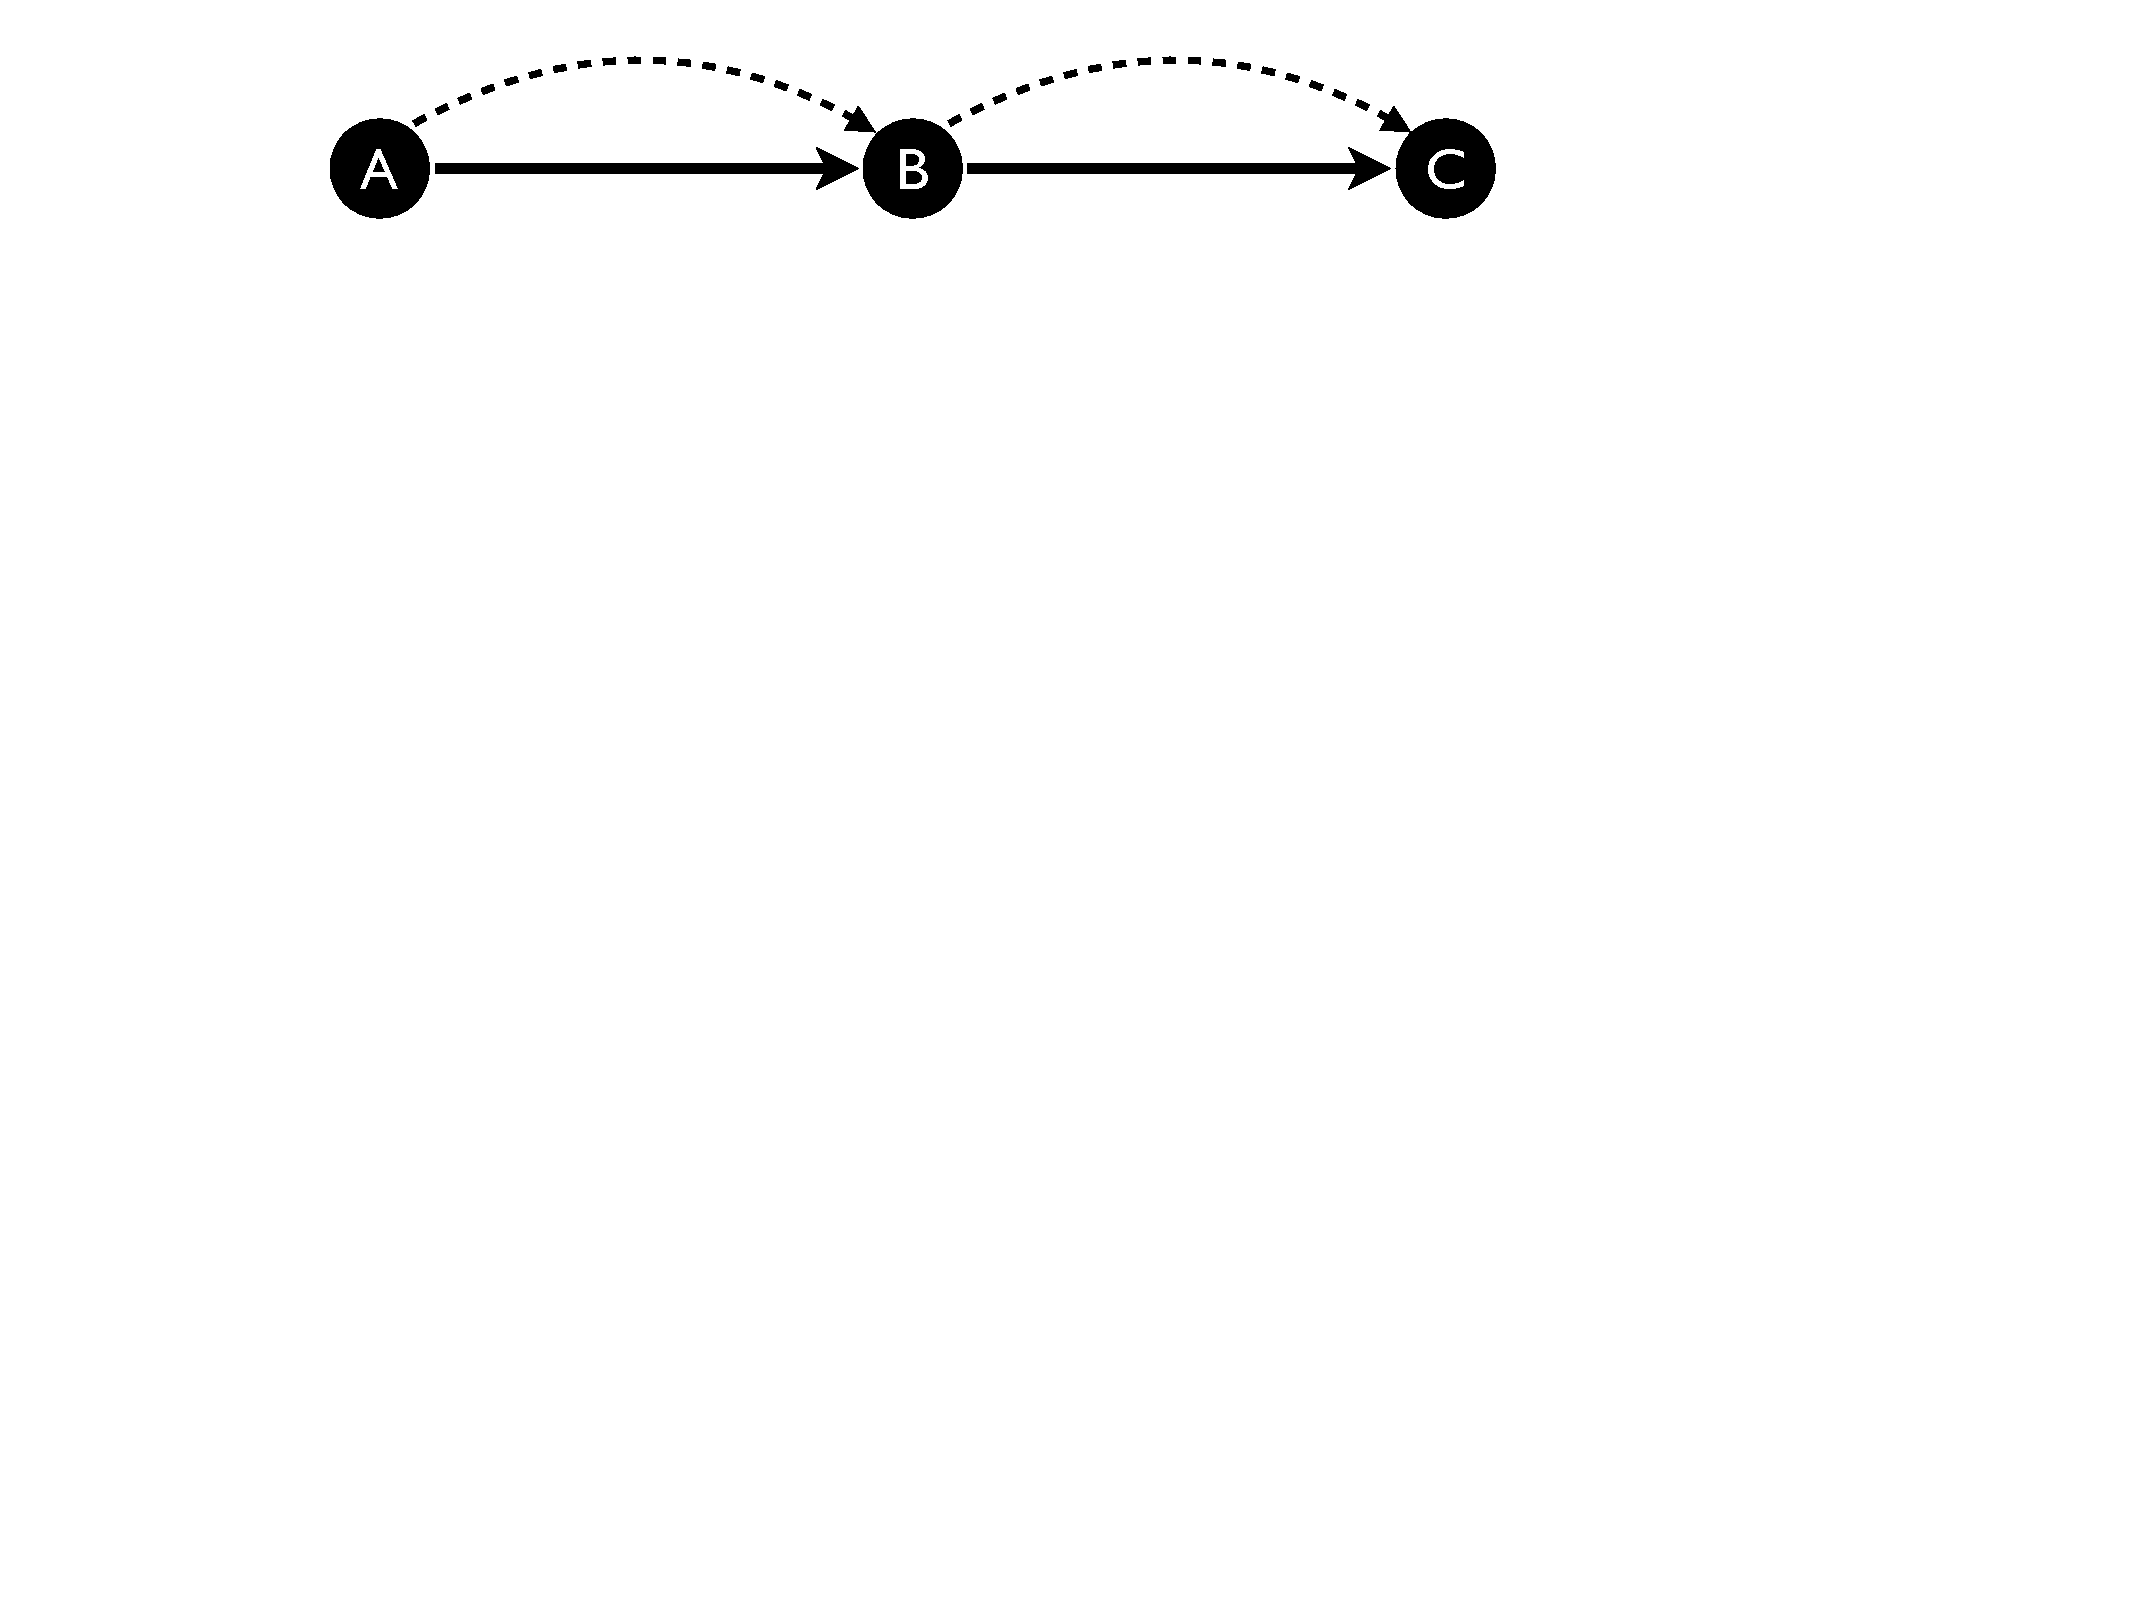
\includegraphics[width=0.5\columnwidth]{figs/seg1}}
  \subfigure[
  Old path: $A \rightarrow B \rightarrow 2 \rightarrow C$, new path: $A \rightarrow 2 \rightarrow B \rightarrow C$. 
  New $AB$ crosses old $BC$, so $AB$ depends on $BC$]{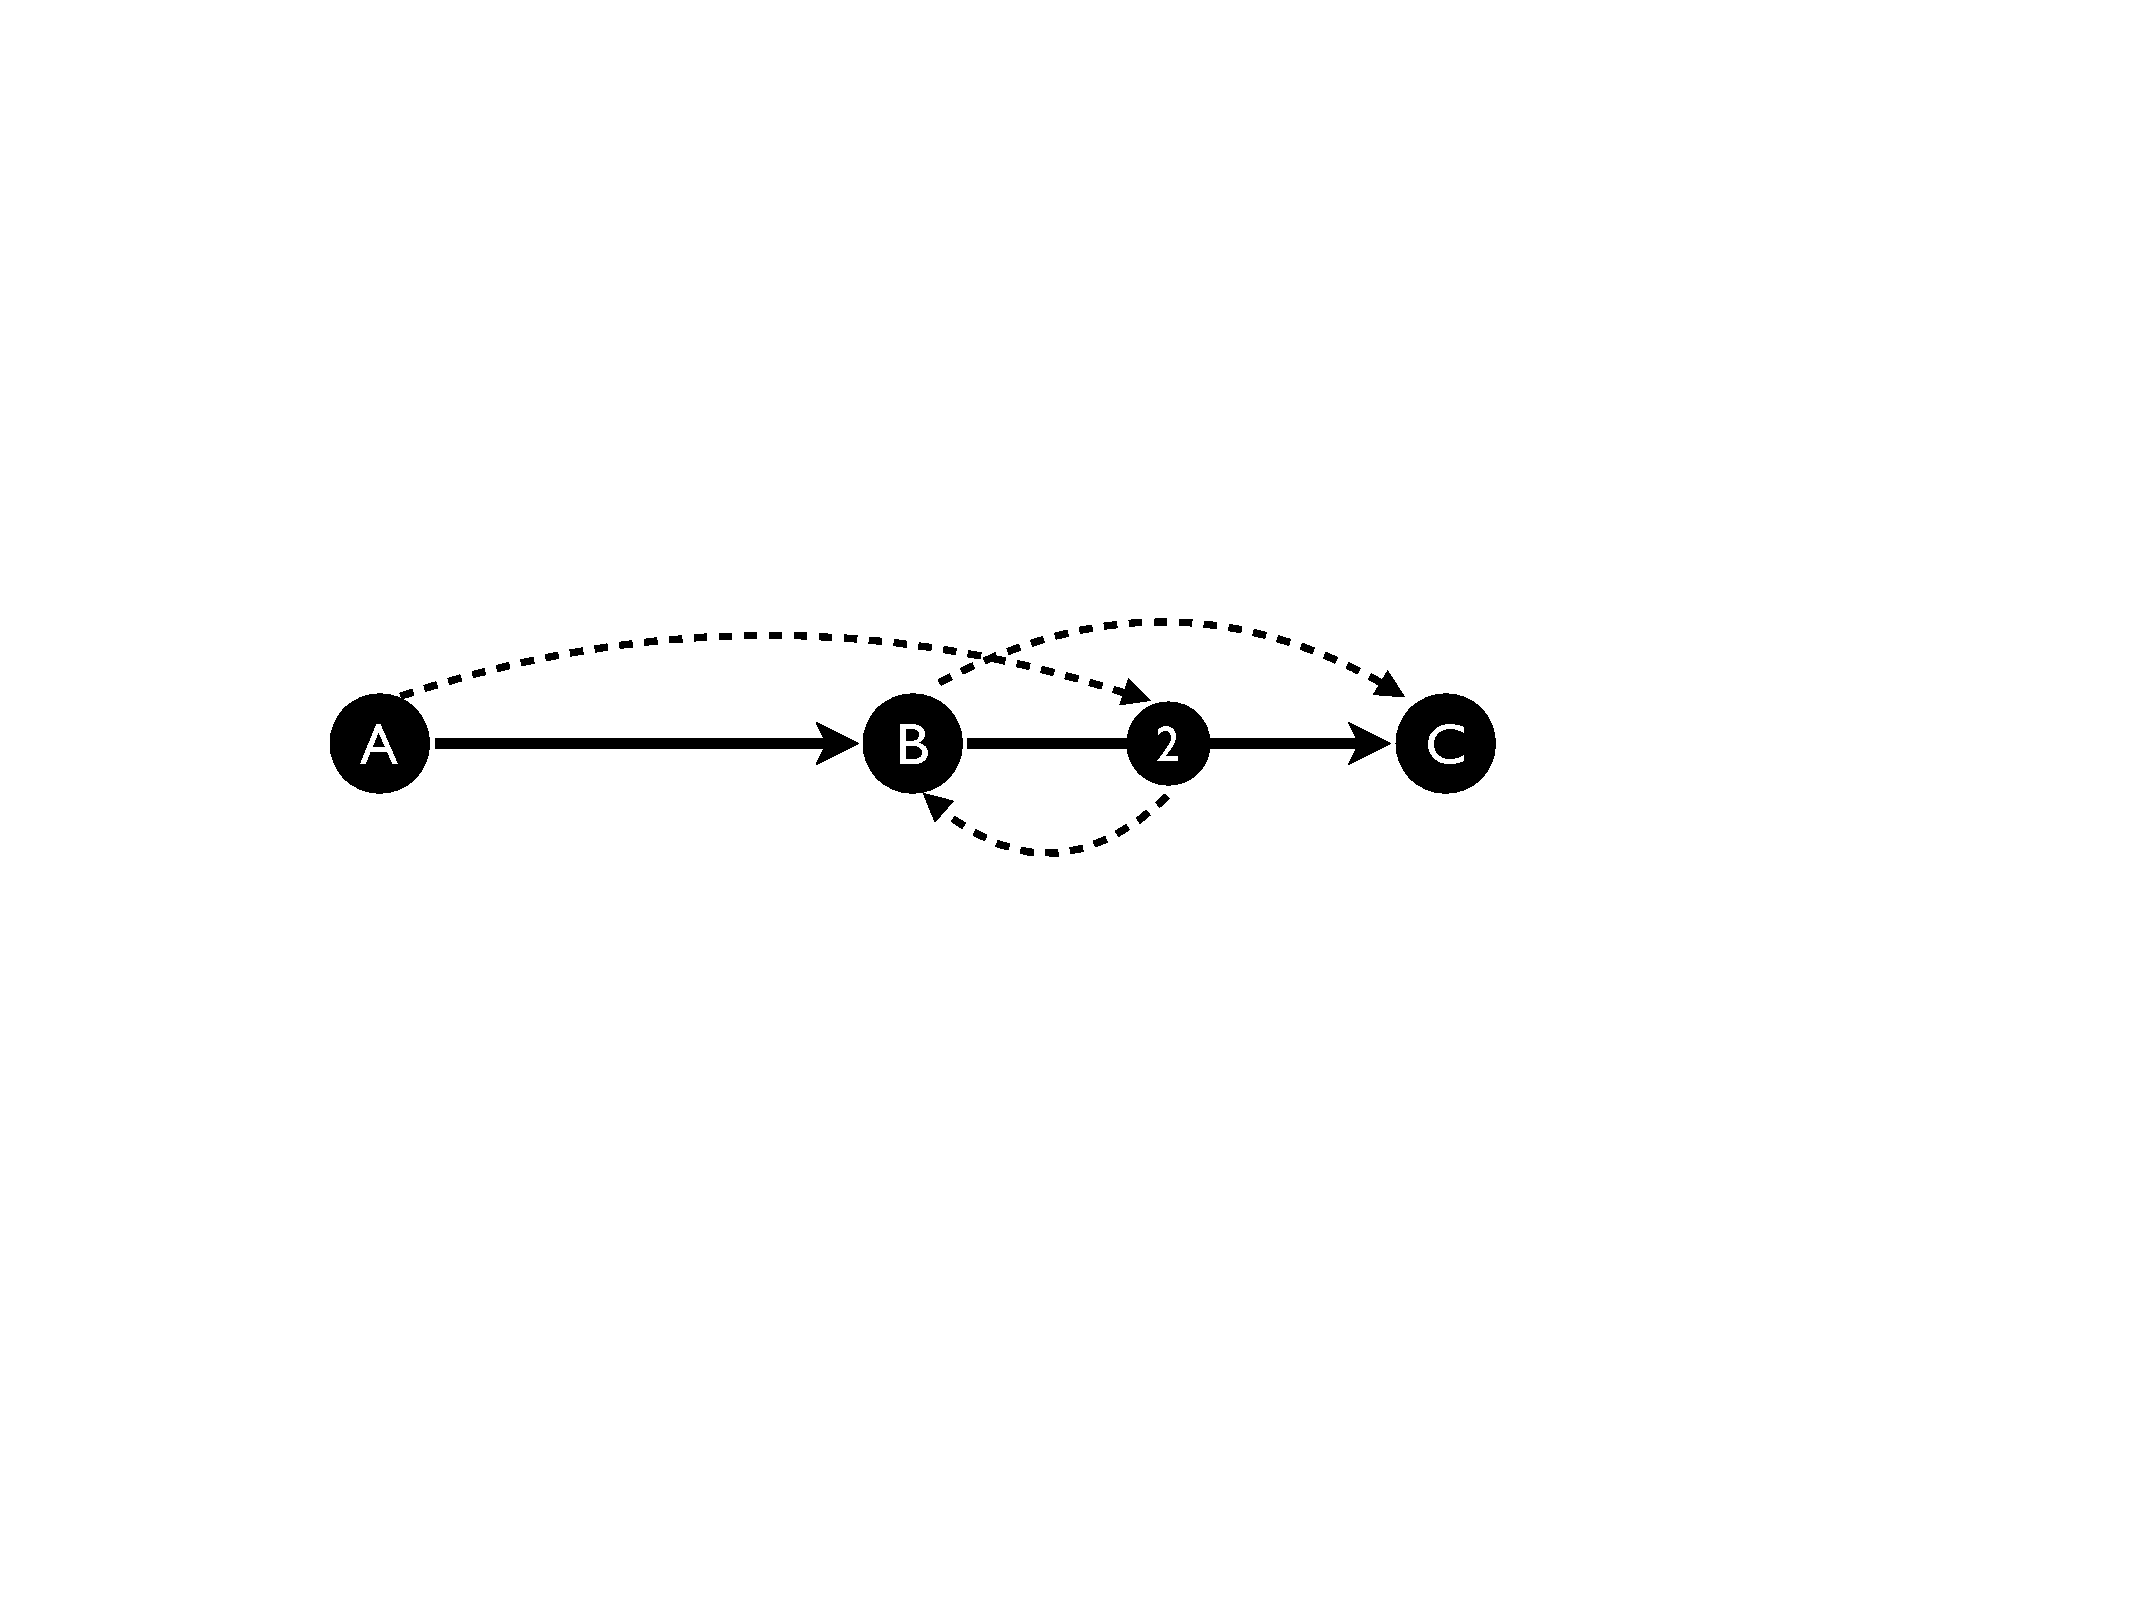
\includegraphics[width=0.5\columnwidth]{figs/seg3}}
  \subfigure[
  Old path: $A \rightarrow 1 \rightarrow B \rightarrow C$, new path: $A \rightarrow B \rightarrow 1 \rightarrow C$. 
  New $BC$ crosses old $AB$, so $BC$ depends on $AB$]{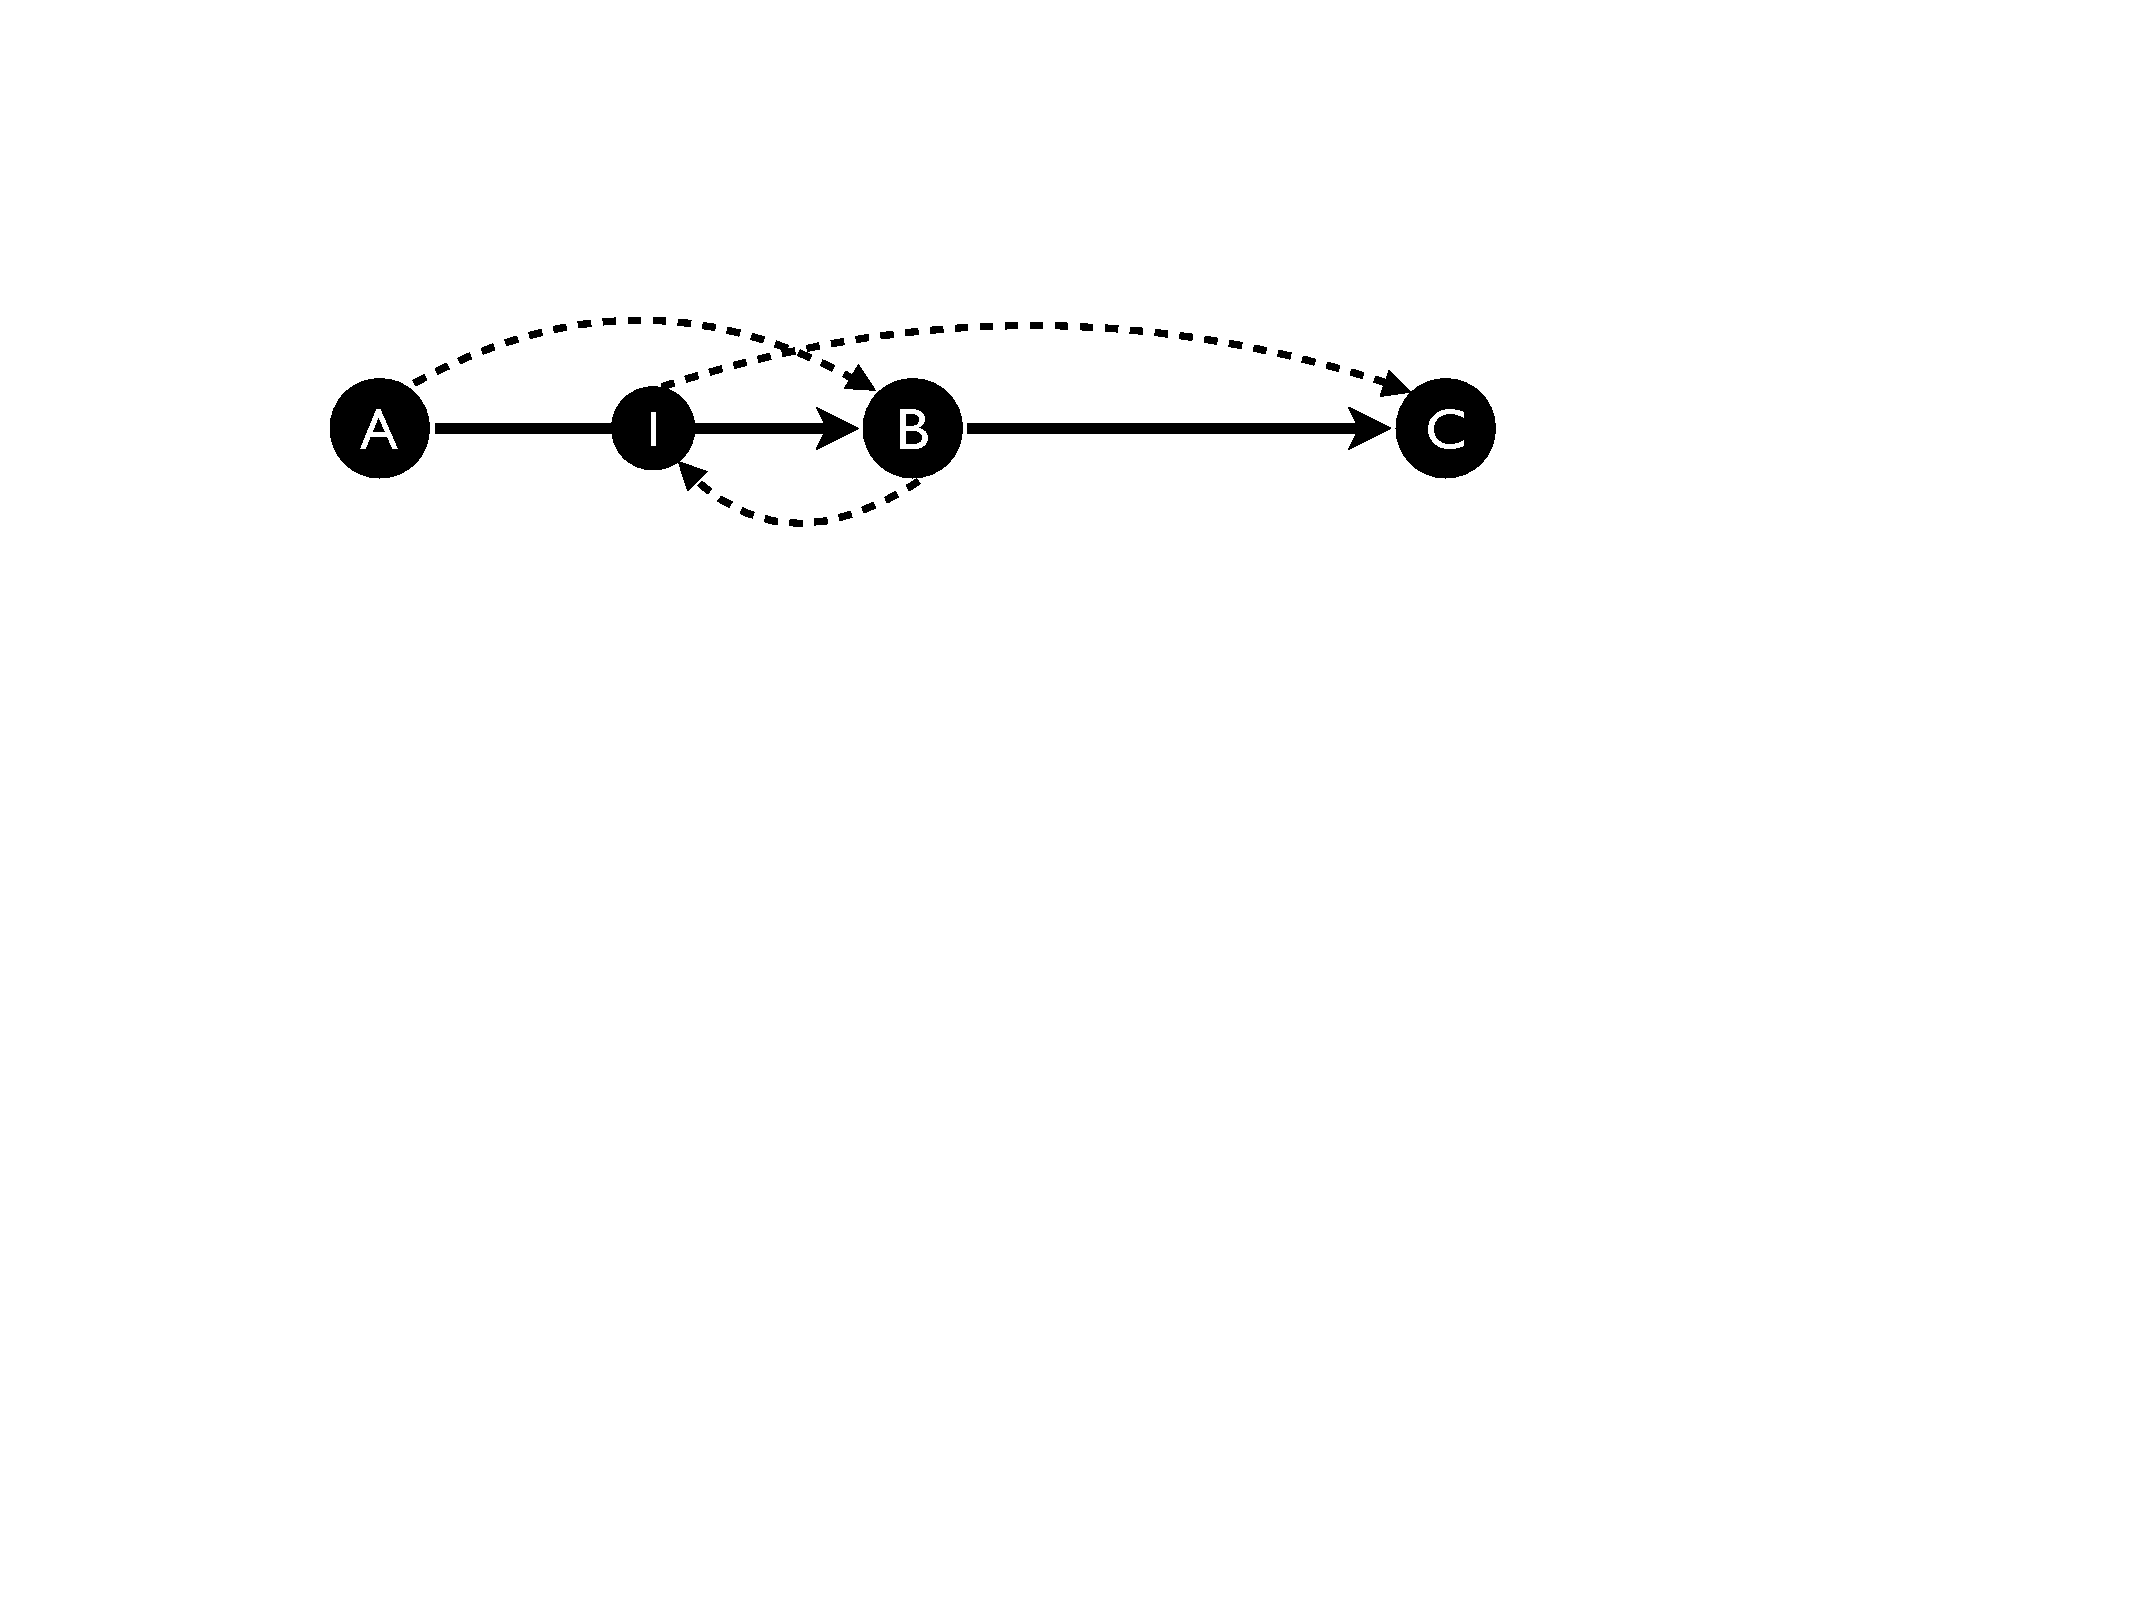
\includegraphics[width=0.5\columnwidth]{figs/seg2}}
  \subfigure[
  Old path: $A \rightarrow \rightarrow 1 \rightarrow B \rightarrow 2 \rightarrow C$, new path: $A \rightarrow 2 \rightarrow B \rightarrow 1 \rightarrow C$. 
  New $BC$ crosses old $AB$, and new $AB$ crosses old $BC$, so $BC$ and $AB$ have circular dependency between themselves.]{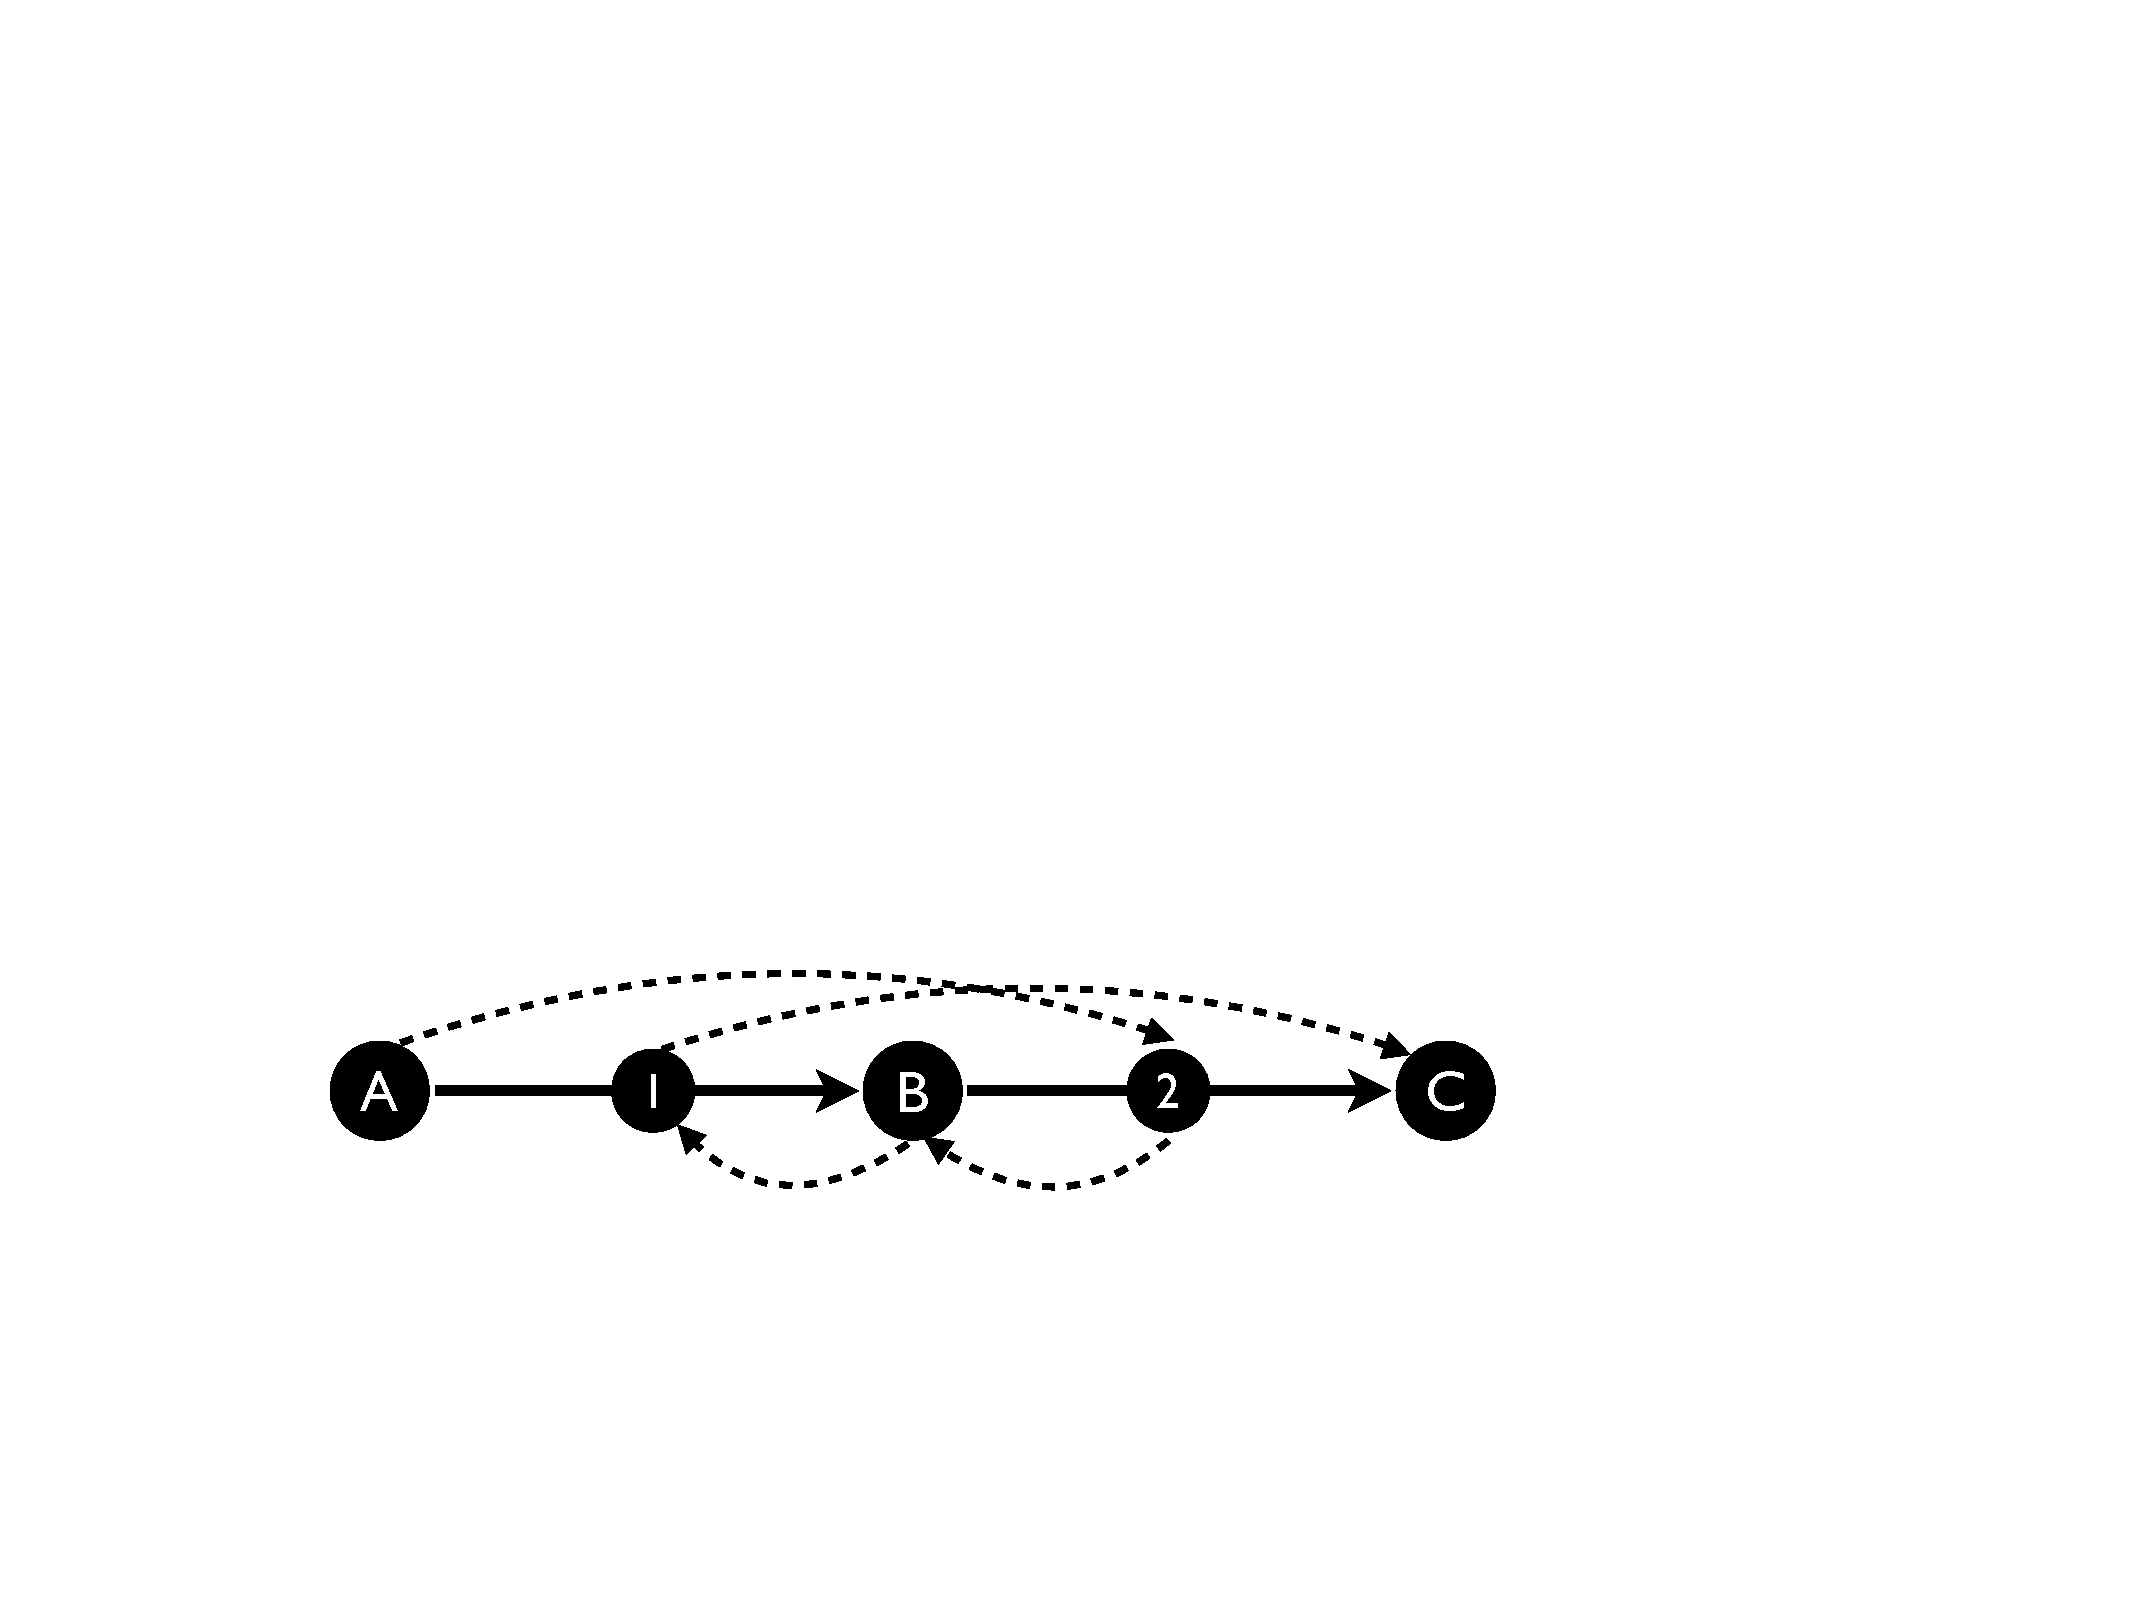
\includegraphics[width=0.5\columnwidth]{figs/seg4}}
  %\subfigure[case 5]{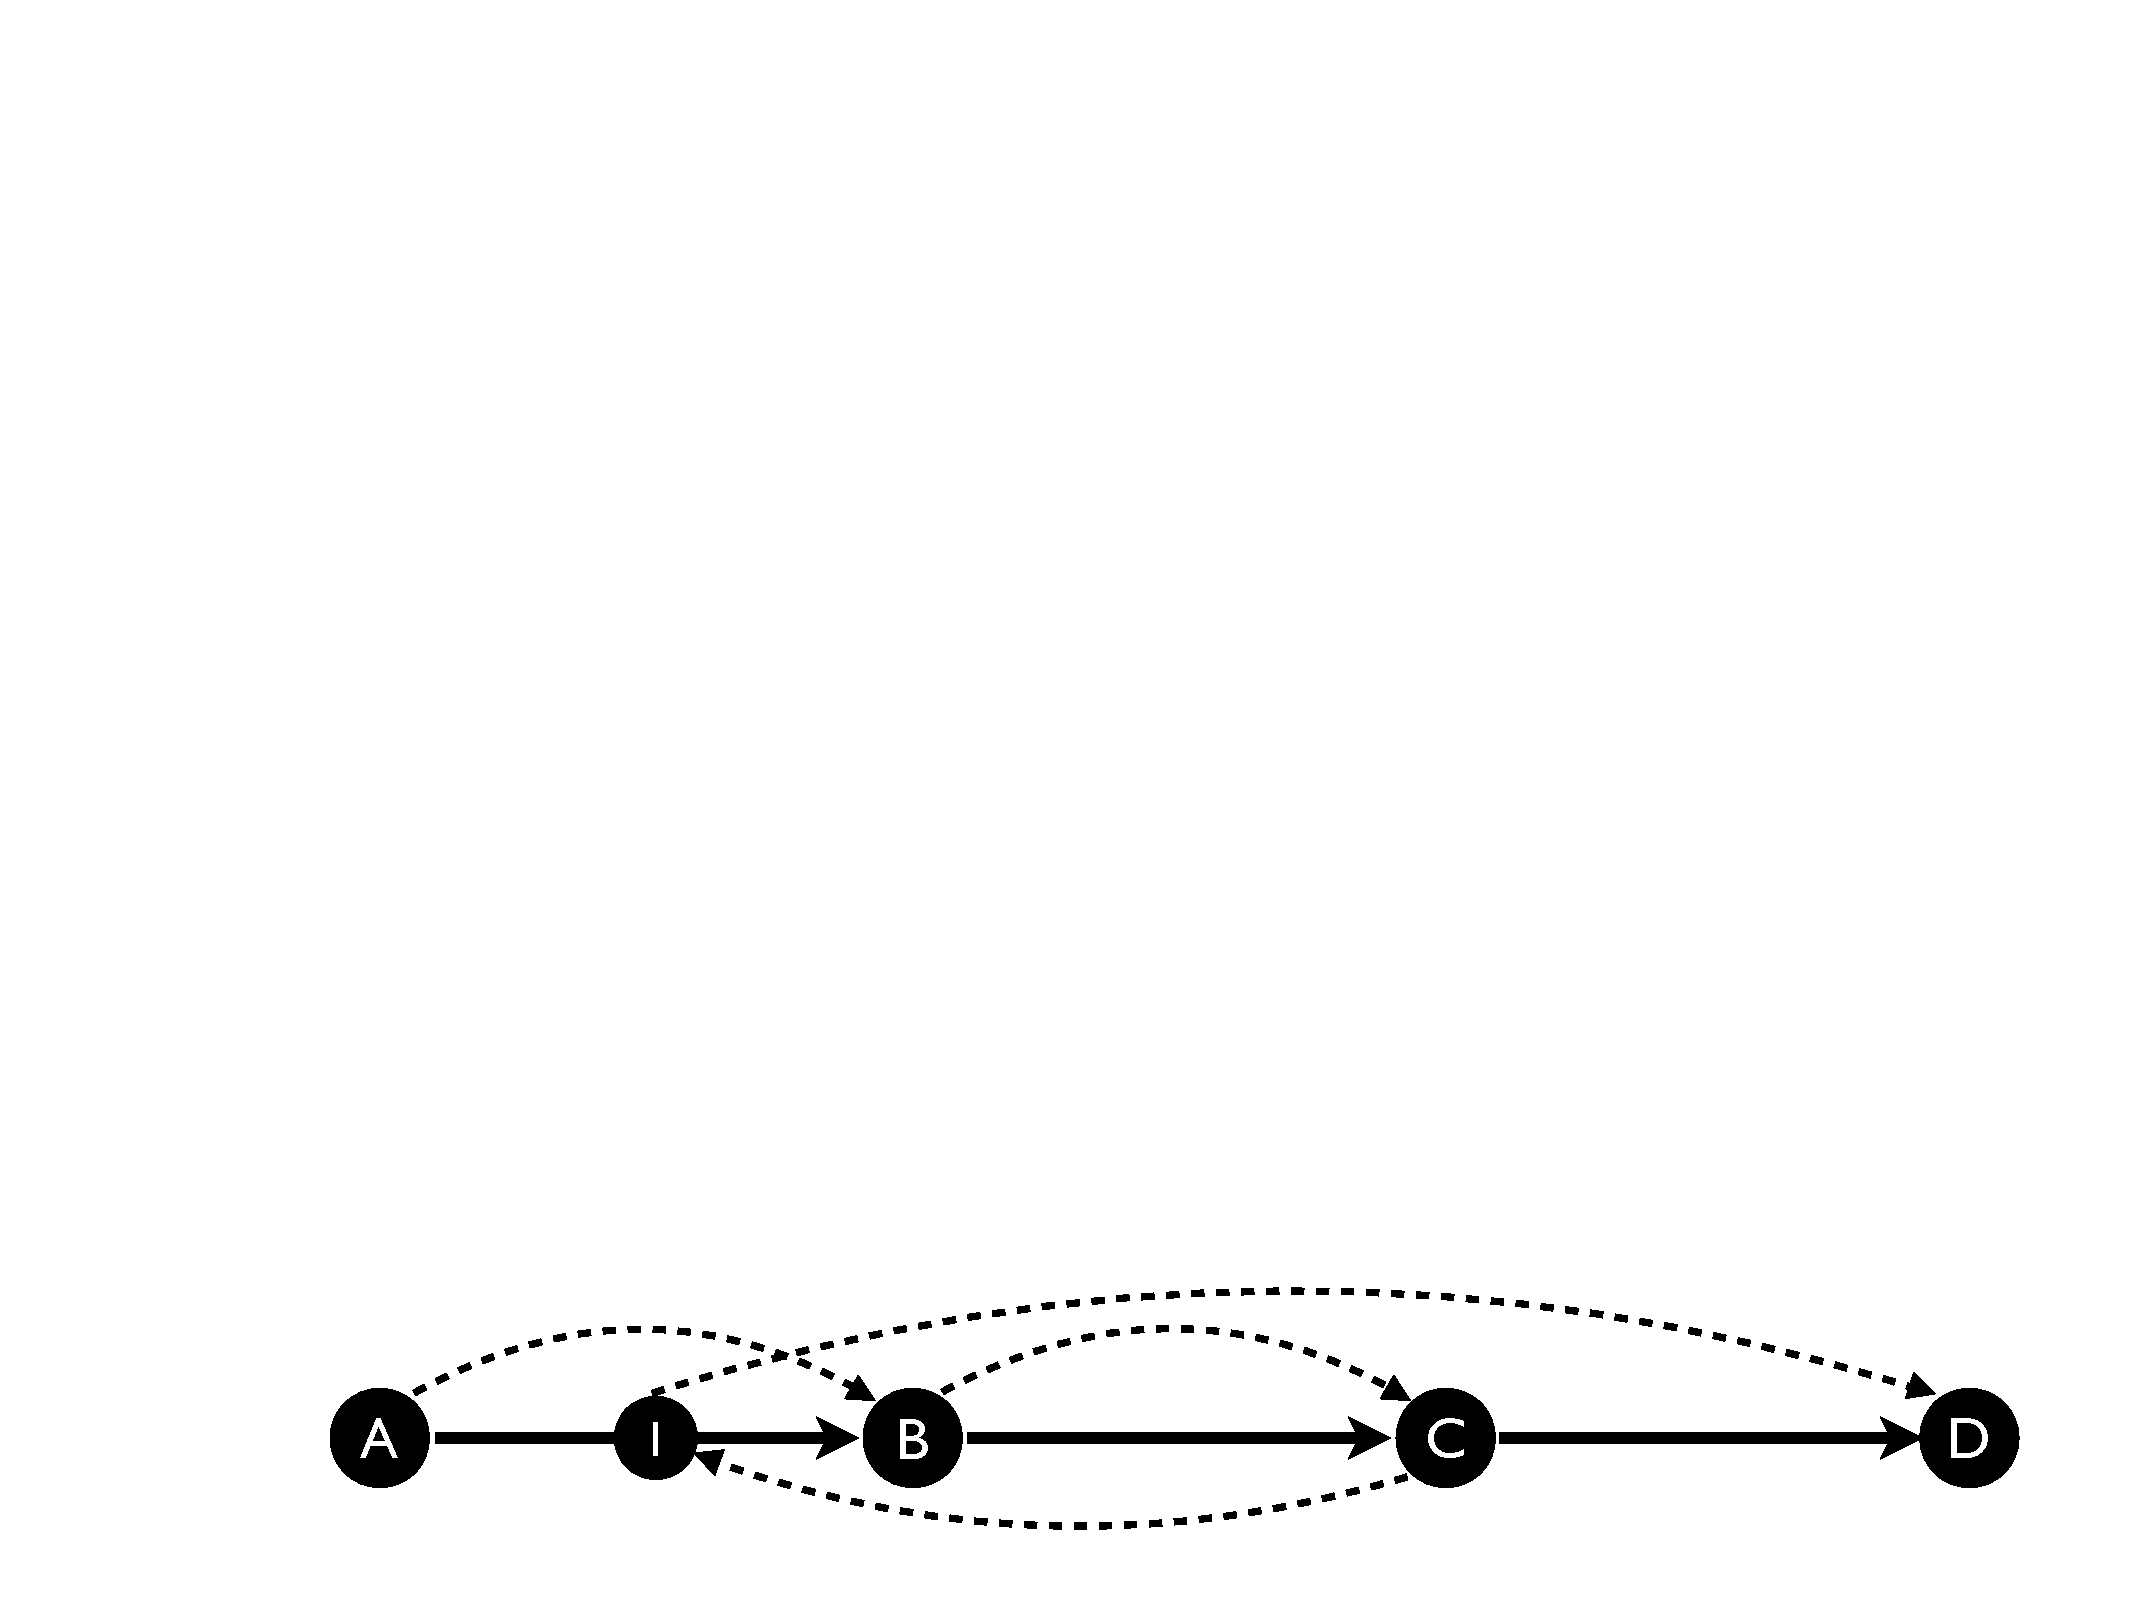
\includegraphics[width=0.7\columnwidth]{figs/seg5}}
  %\vspace{10pt}
  \vspace{-0.2in}
  \caption{\em \small Examples: dependencies between segments. Path $AC$ is divided into two segments $AB$ and $BC$ by three waypoints $A$, $B$, and $C$, with old paths in solid lines, and new paths in dashed lines. \kevinc{changes in the subtitle to clearly specify the new/old path} }
  \vspace{-0.2in}
  \label{fig:circular}
\end{figure*}

  \vspace{-0.1in}
\begin{theorem} If there is no circular dependency between segments, then an update order that preserves the required property always exists. 
In particular, if policies are enforcing no more than two waypoints,
an update order always exists. 
%\begin{itemize}[noitemsep,topsep=0pt,leftmargin=*]
%\item independent ECs, i.e., no overlapping updates across different ECs.
%\item no circular dependencies between segments. 
%In particular, if invariants are enforcing no more than two waypoints.
%an update order always exists. 
%\end{itemize} 
\end{theorem}
  \vspace{-0.1in}

If a policy introduces no circular dependency, 
i.e., at least one segment can be updated independently (Figure~\ref{fig:circular}(a-c)), 
then we say the policy is {\em segment independent}.
%Figure~\ref{fig:circular}(a) shows us one such example. 
However, in reality, forwarding links and paths may be shared by different sets of packets, e.g., multiple flows. Thus it is possible that two forwarding links (smallest possible segments) $l_1$ and $l_2$ will have 
conflicting dependencies when serving different groups of packets, e.g., in forwarding graphs destined to two different IP prefixes. In such cases, circular dependencies are formed across forwarding graphs. 
Fortunately, forwarding graphs do not share links in many cases. 
For example, as pointed out in~\cite{jin2014dynamic}, a number of flow-based traffic management applications 
for the network core (e.g., ElasticTree, MicroTE, B4, SWAN~\cite{microte, heller2010elastictree, jain2013b4, Hong13}), any forwarding rule at a switch matches at most one flow.

%\wxzc{need to prove it holds for multi-path?}

\paragraph{Other Properties}

There are trace properties which are not waypoint-based, such as
quantitative properties like path length constraint. 
To preserve such properties and waypoint-based trace properties that are not segment independent,
\kevin{we can use other heavyweight techniques as a fallback (see \ref{sec:synthesis}), such as CU~\cite{Reitblatt2012}.}
%\name is plugged in with CU~\cite{Reitblatt2012} as backup to its heuristic component. 
Besides, there are network properties beyond trace properties, such as congestion freedom,
%\cut{quality of service, and }congestion freedom. 
%Among those, congestion freedom is a common and important one. 
and it has been proven that careful ordering of updates cannot always guarantee congestion freedom~\cite{Hong13, loopfree-flow}. 
\kevin{To ensure congestion freedom, one approach is to use other heavyweight tools, such as SWAN~\cite{Hong13}, as a fallback mechanism that the default heuristic algorithm can trigger only when necessary.}

%we plug in a heavyweight tool (e.g., SWAN, which is the one used in our implementation) to work together with the heuristic algorithm.  

%Overlapping ECs:
%1. split updates to non-overlapping; 2. use mechanisms like CU.

%Slice isolation: If the output
%of packet set of slice $a$ at any switch port, overlaps with any other slice,
%then there is the potential for leaks. 
%
%Multiple waypoints 

%Path length constraint: Suppose
%we wish to ensure that no flow from port $C$ to port $S$ should go through more
%than 3 switches represents this check.
%
%Quantitative properties (with SWAN)                         

\subsection{Consistency Preserving Network Synthesis}
\label{sec:synthesis}

\wxznew{ 
%\cut{As discussed previously, there may be situations in which this
%greedy algorithm gets stuck, i.e., some buffered updates never pass the
%verification.  That may happen }
When desired policies do not have the segment-independence property (\S\ref{sec:seg-independence}), it is possible that some buffered updates (through very rare in practice) never pass the verification.}
%\cut{ using the greedy algorithm}
For instance, consider a circular network with three nodes, in which each node
has two types of rules: one type to forward packets to destinations directly connected to itself, and one default rule, which covers destinations connected to the other two switches. 
Initially, default rules point clockwise. They later change to
point counter clockwise. No matter which of the new default
rules changes first, a loop is immediately caused for some destination. 
\wxzcr{The loop freedom property is not segment-independent in this case, because that each default rule
is shared by two flows (destined to two hosts),
which results in conflicting dependencies among forwarding links.}
To handle scenarios like that, 
we adopt a hybrid approach (Algorithm 2).  If the network
operators desire some policies that can be guaranteed by existing
solutions, e.g., CU or SWAN, such solutions can be specified and plugged in as
the fallback mechanism, $FB$.
The stream of updates is first handled by \name's greedy heuristic (Algorithm 1)
%from the application is first fed into the translation layer to be transformed
%to a feasible update sequence. Then \name greedily sends updates
as long as the
policy is preserved. Updates that violate the policy are buffered temporarily.
When the buffering time is over threshold $T$, configured by the operator,
the fallback mechanism is triggered.
The remaining updates are fed into $FB$ to be transformed to a feasible sequence, and then Algorithm 1 proceeds with them again to heuristically maximize update parallelism. 
In that way, \name can always generate a consistent update sequence.
%\cut{avoids getting stuck.}
Alternatively, if no such external mechanism exists, 
\kevinc{prefer to remove ``if no such external mechanism exists"} or the operators highly
value update efficiency and prefer a best effort mechanism to maintain consistency
during updates, no fallback would be triggered and no
$FB$ would be provided to the algorithm.  Instead, after a
configurable threshold of time, buffered commands are released to the network.
\wxzcr{Thus, all updates are guaranteed to be issued eventually either way.}
%Such design gives operators a flexible choice on how to balance the trade-off between efficiency and consistency.
\wxzcr{Note that even with $FB$ triggered, \name achieves better efficiency 
than using $FB$ alone to update the network,
because: 1) in the common case, most of updates are not handled by $FB$;
2) \name only uses $FB$ to "translate" buffered updates and then 
heuristically parallelize issuing the output of $FB$, 
but doesn't wait explicitly as some $FB$ mechanism does, e.g., the waiting time between two phases in CU.}

%  \vspace{-0.1in}
\begin{algorithm}[t]
  \small
\caption{Synthesizing update orderings}
\bf{ScheduleUpdates}($Model, Buf, U, FB, T$)
\begin{algorithmic} 
\For {$u \in U$}
        \State \bf{ScheduleIndividualUpdate($Model, Buf, u$)}
\EndFor
\State 
\State \bf{On timeout($T$):}
\State $\tilde{U}$ = \bf{Translate($Buf, FB$)}
\For {$u \in \tilde{U}$}
        \State \bf{ScheduleIndividualUpdate($Model, Buf, u$)}
\EndFor
\label{alg:synthesize}
\end{algorithmic}  
\end{algorithm}

\if 0
\begin{figure}[!ht]
  \centering
  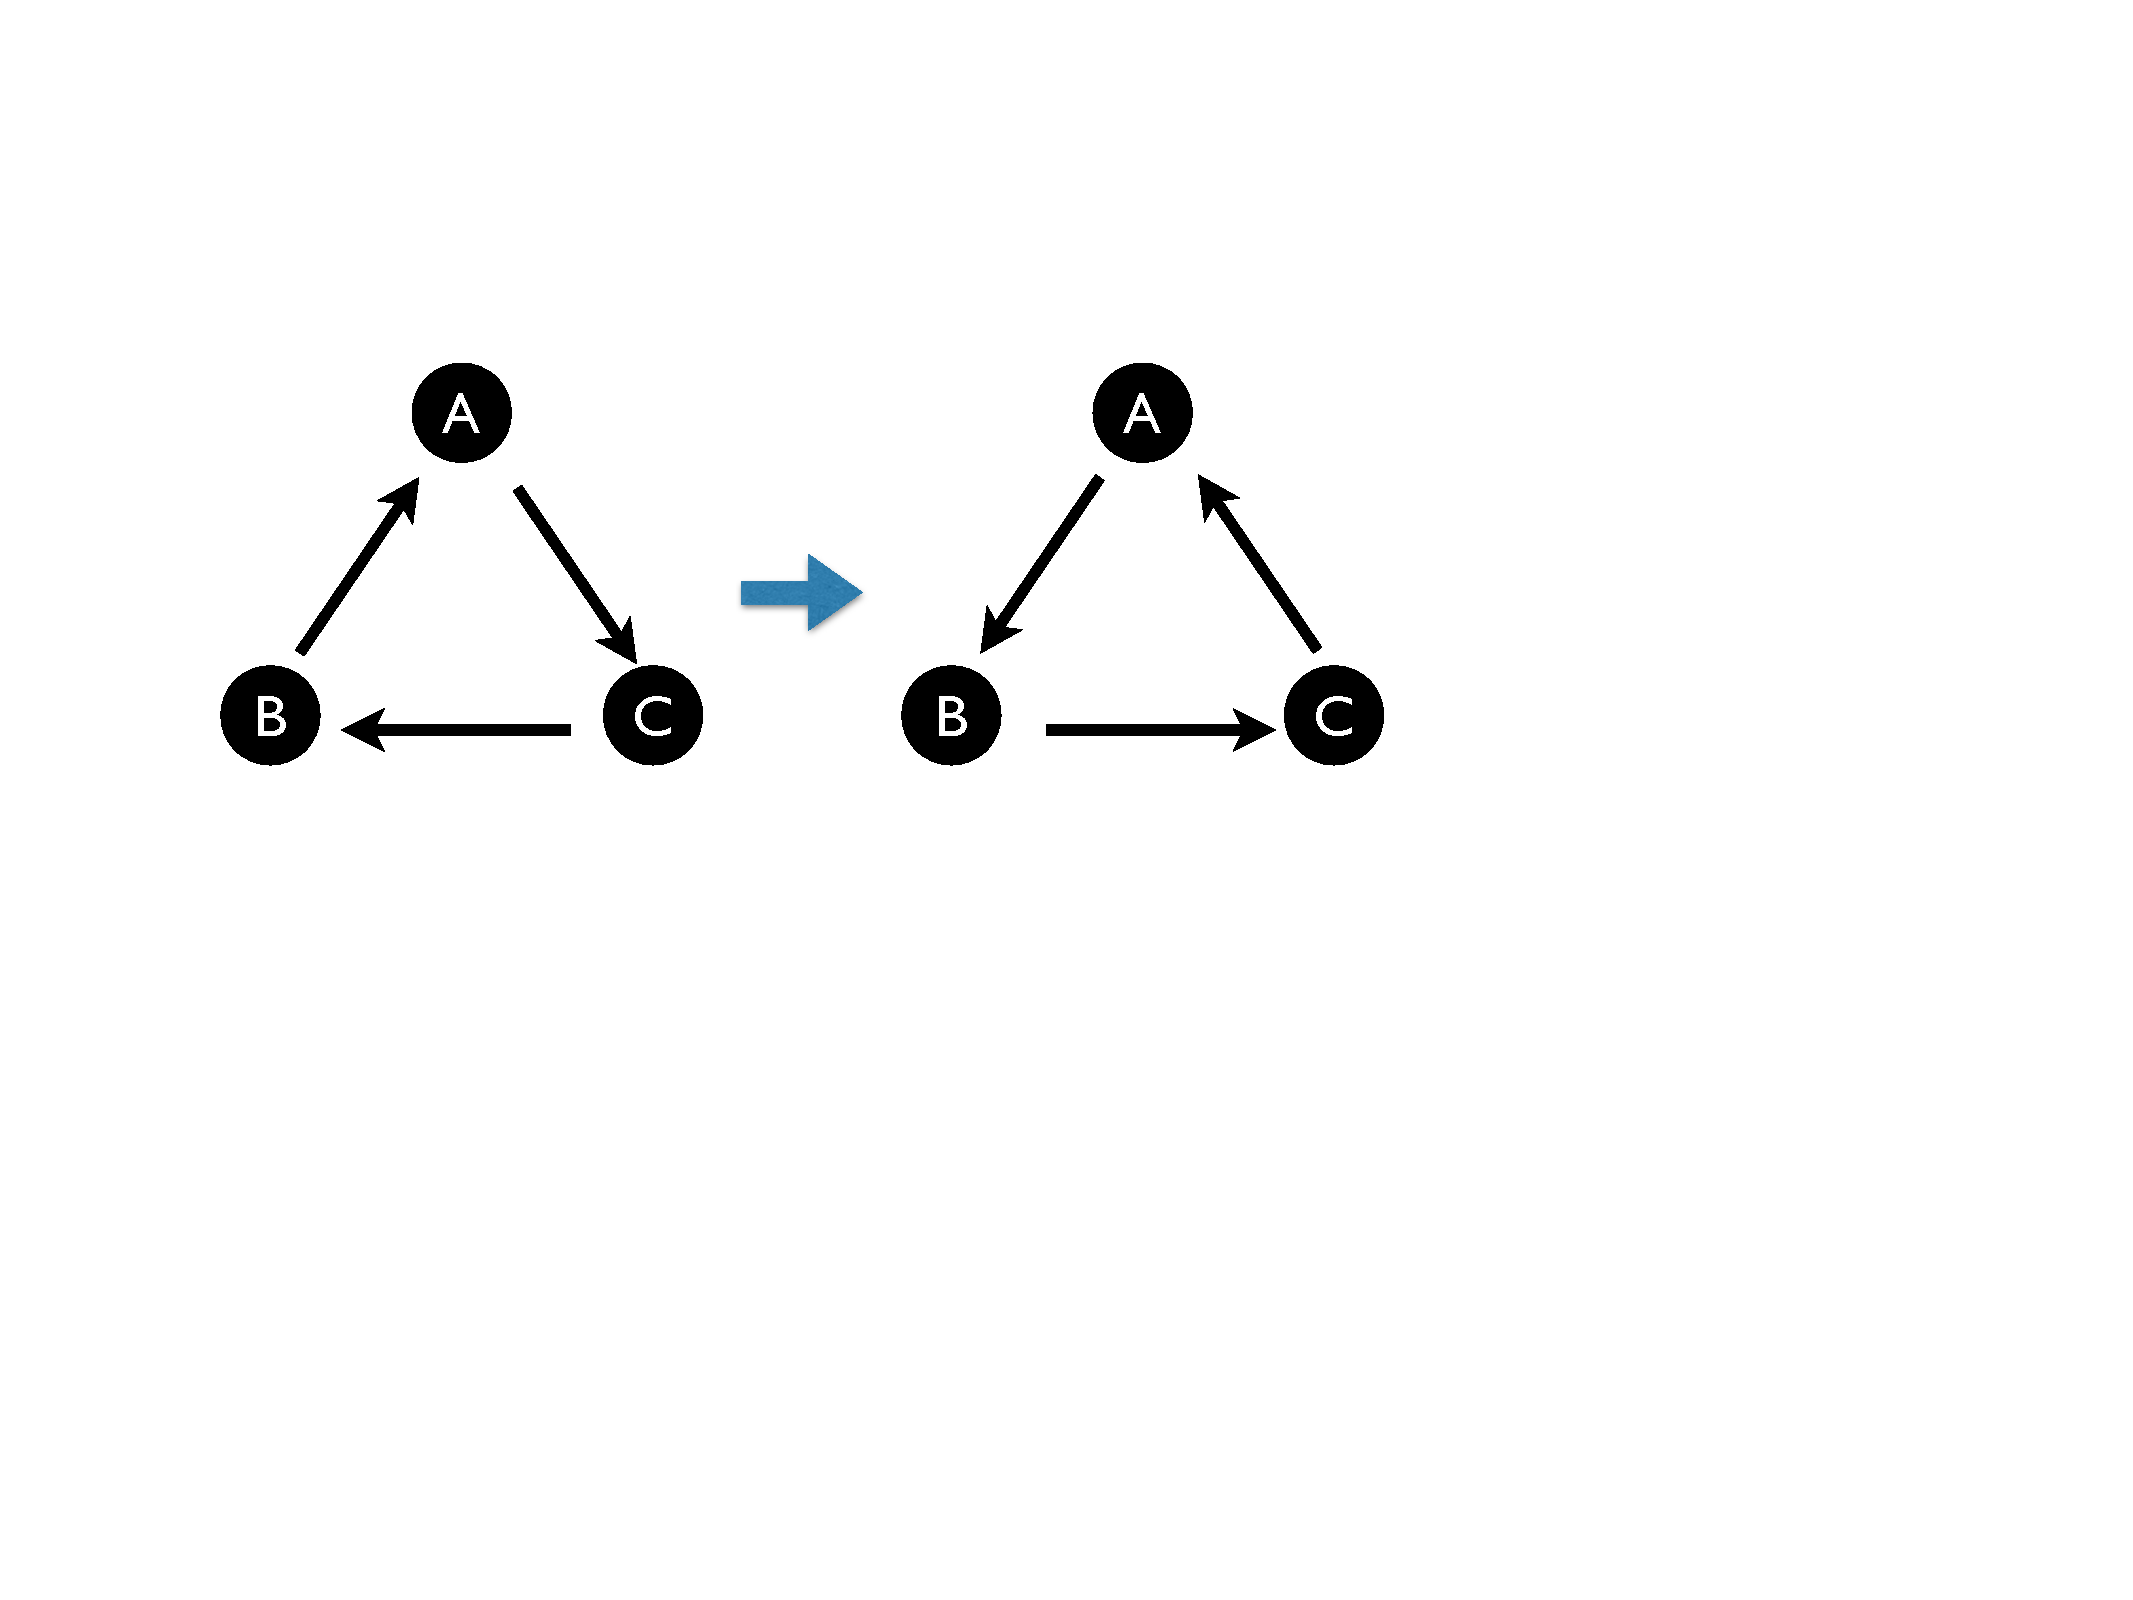
\includegraphics[width=0.7\columnwidth]{figs/triangle}
  \caption{\em \small Illustrating case where Algorithm1 gets stuck.}
  \label{fig:example}
\end{figure}
\fi

To show the feasibility of that approach,
%\cut{we integrated \name with both CU \cite{Reitblatt2012} and SWAN \cite{Hong13} as plug-ins.} 
\kevin{we implemented both CU \cite{Reitblatt2012} (see \S\ref{sec:eval}) and SWAN \cite{Hong13} as our fallback mechanisms in \name.}
%\cut{The integration with CU is thoroughly evaluated in \S\ref{sec:eval}, and here, we focus on the one with SWAN. } 
%We verified congestion-free invariants of 
We emulated traffic engineering (TE) and failure recovery (FR), similar to Dionysus \cite{jin2014dynamic}, in the network shown in Figure \ref{fig:swan_topo}. Network updates were synthesized to preserve congestion-free property using \name (with SWAN as plug-in), and for comparison, using SWAN alone. In the TE case, we changed the network traffic to trigger new routing updates to match the traffic. In the FR case, we turned down the link S3-S8 so that link S1-S8 was overloaded. Then the FR application computed new updates to balance the traffic.
 %and eventually eliminate the link overload. 
The detailed events that occurred at all eight switches are depicted in Figure \ref{fig:bw}. We see that \name ensured the same consistency level, but greatly enhanced parallelism, and thus achieved significant speed improvement (1.95x faster in the TE case, and 1.97x faster in the FR case).

\begin{figure}[!ht]
  \centering
  \vspace{-0.1in}
  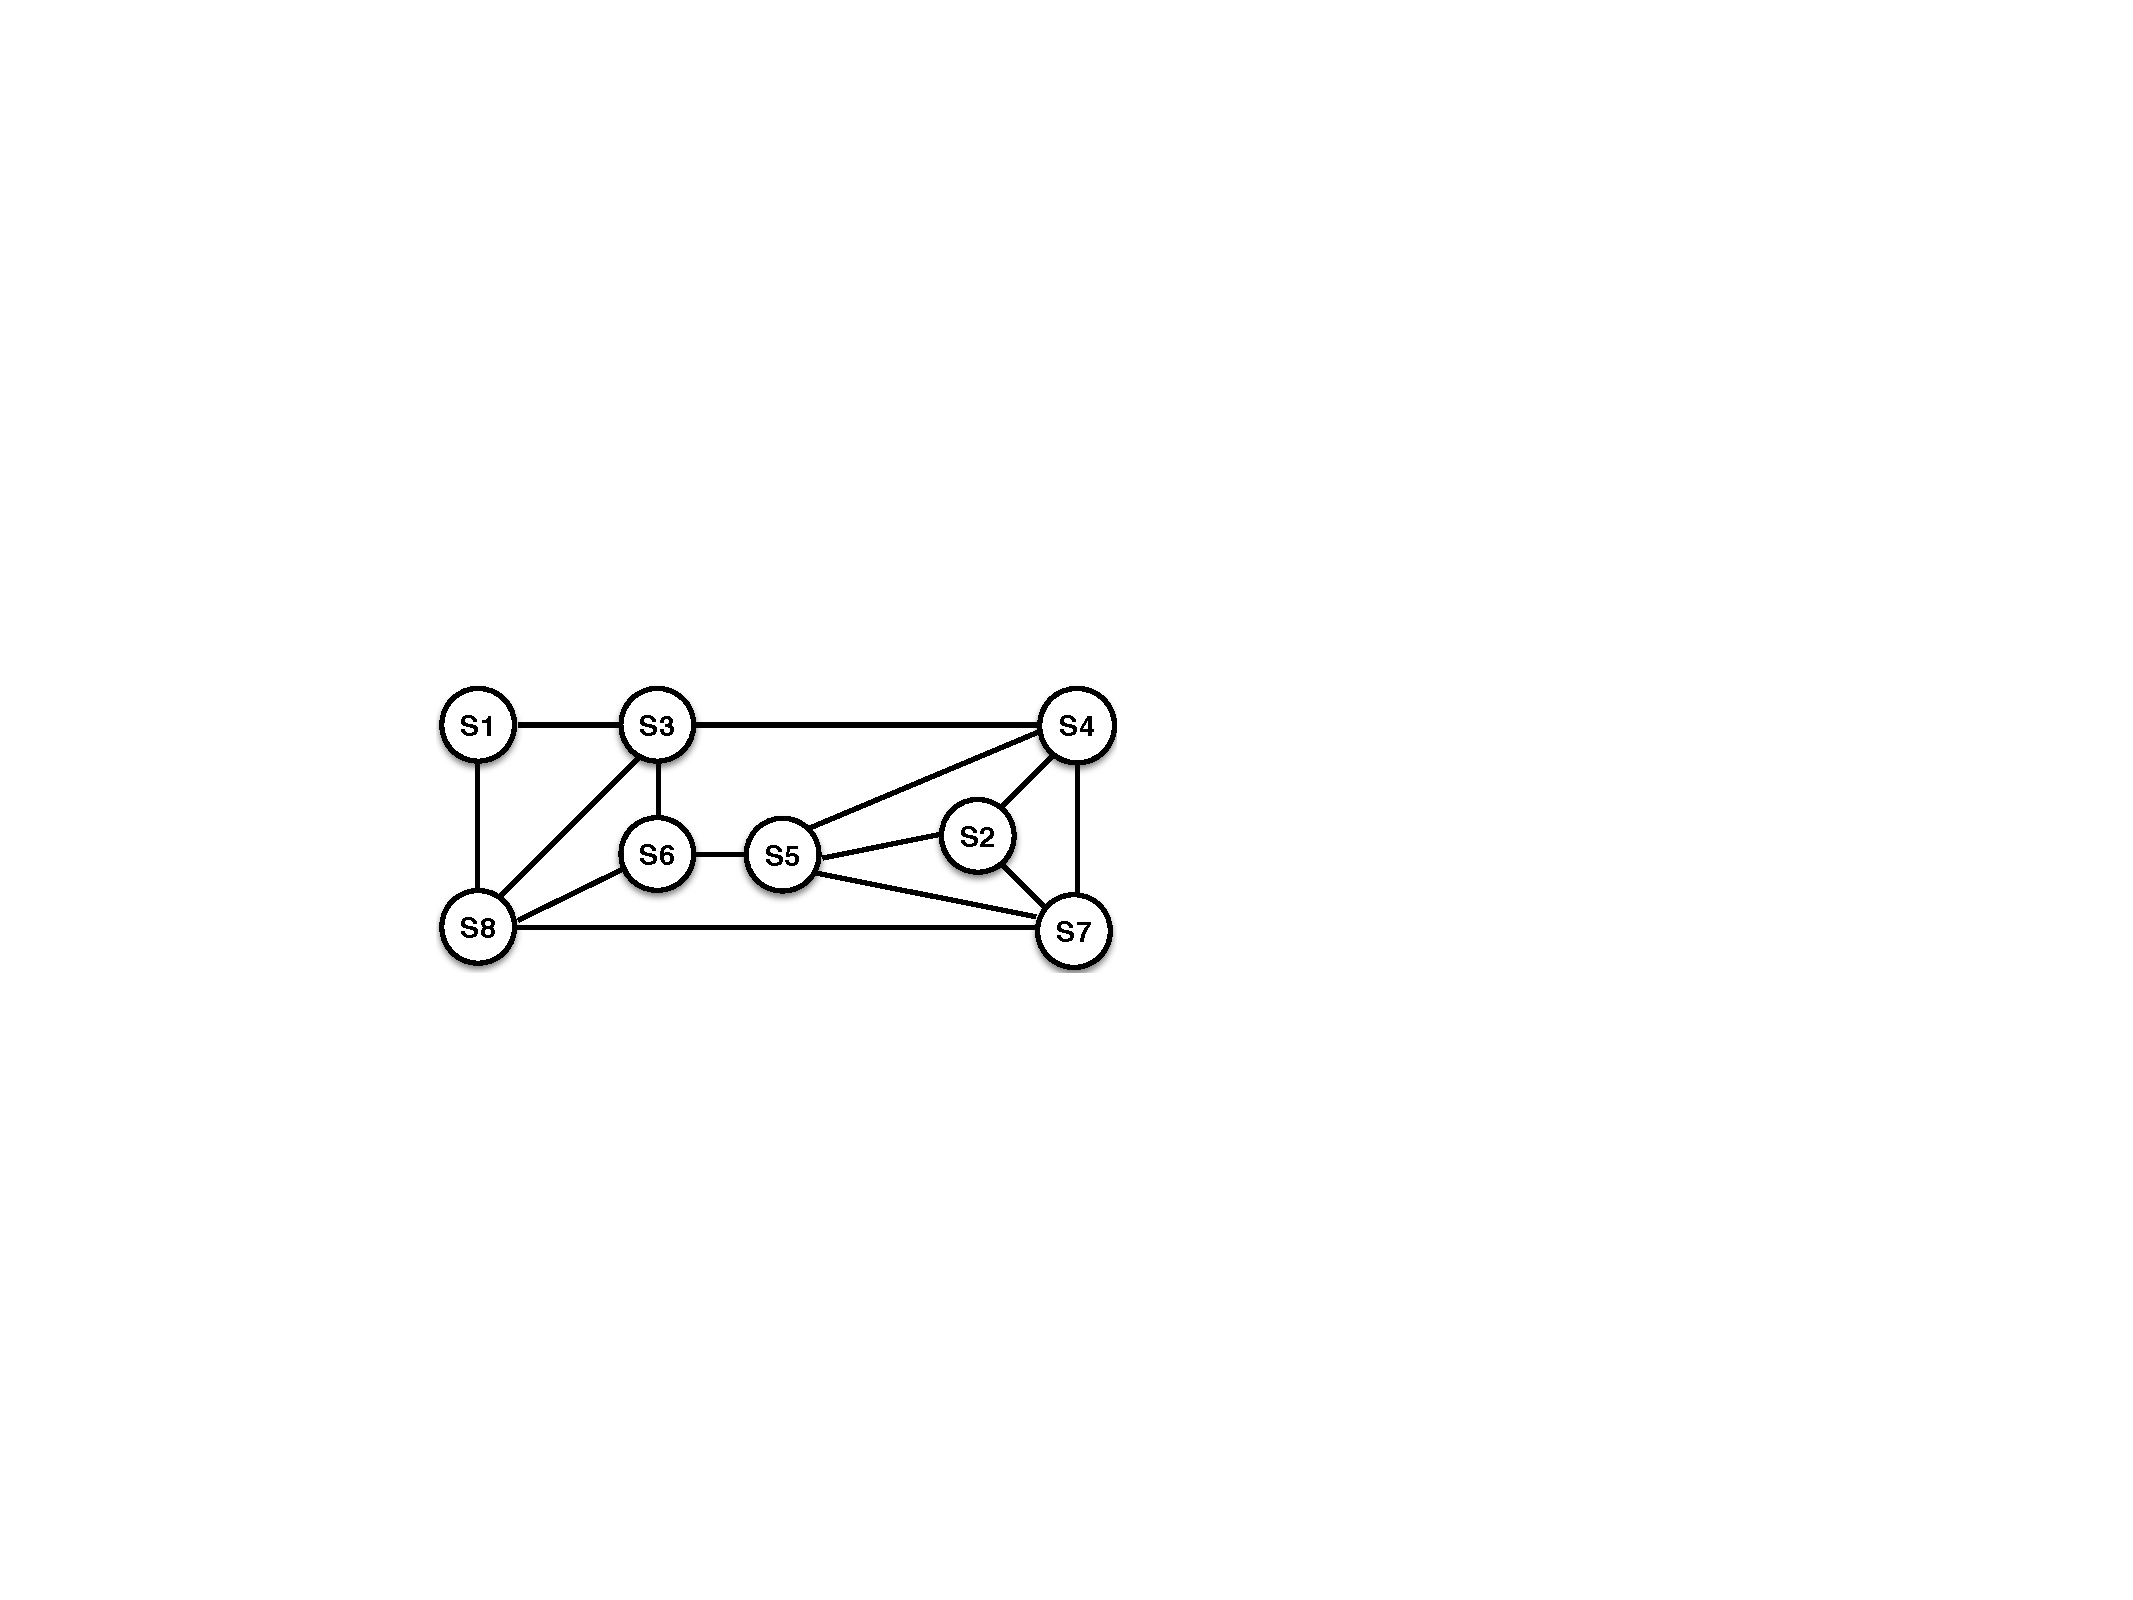
\includegraphics[width=0.5\columnwidth]{figs/swan_topo}
  \vspace{-0.12in}
  \caption{\em \small Topology for \name and SWAN bandwidth tests}
  \vspace{-0.25in}
  \label{fig:swan_topo}
\end{figure}

\cut{
\begin{figure*}[!ht]
  \centering
  \vspace{-0.1in}
  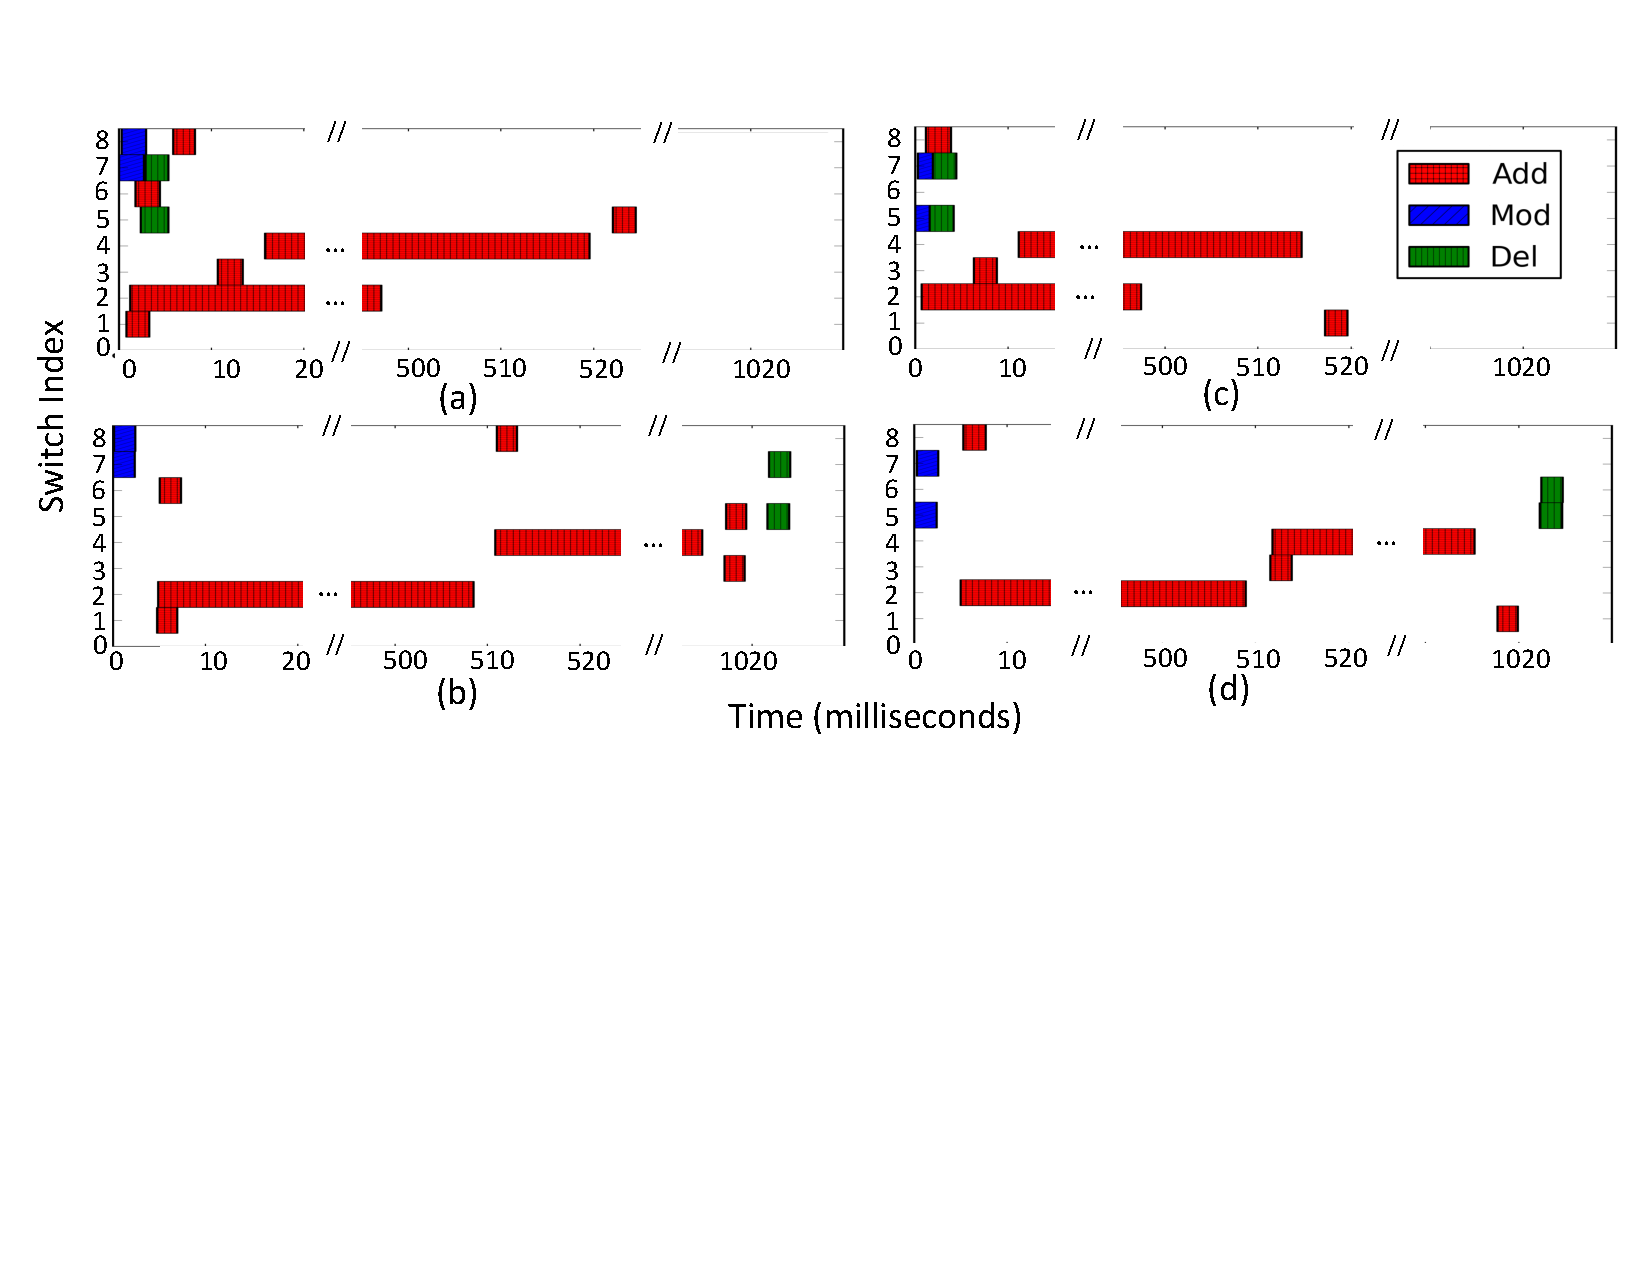
\includegraphics[width=0.8\textwidth]{figs/bandwidth}
  \vspace{-0.1in}
  \caption{\em Time series of events that occurred across all switches: (a) SWAN + \name, traffic engineering; (b) SWAN, traffic engineering; (c) SWAN + \name, failure recovery; (d) SWAN, failure recovery.}
  \vspace{-0.2in}
  \label{fig:bw}
\end{figure*}
}

 \begin{figure*}
        \begin{minipage}[b]{1.2in}
        \caption{\label{fig:bw}\em Time series of events that occurred across all switches: (a) SWAN + \name, traffic engineering; (b) SWAN, traffic engineering; (c) SWAN + \name, failure recovery; (d) SWAN, failure recovery. In both cases, \name + SWAN finishes about 2x faster.}
        \end{minipage}
        \hfill
        \begin{minipage}[b]{6in}
        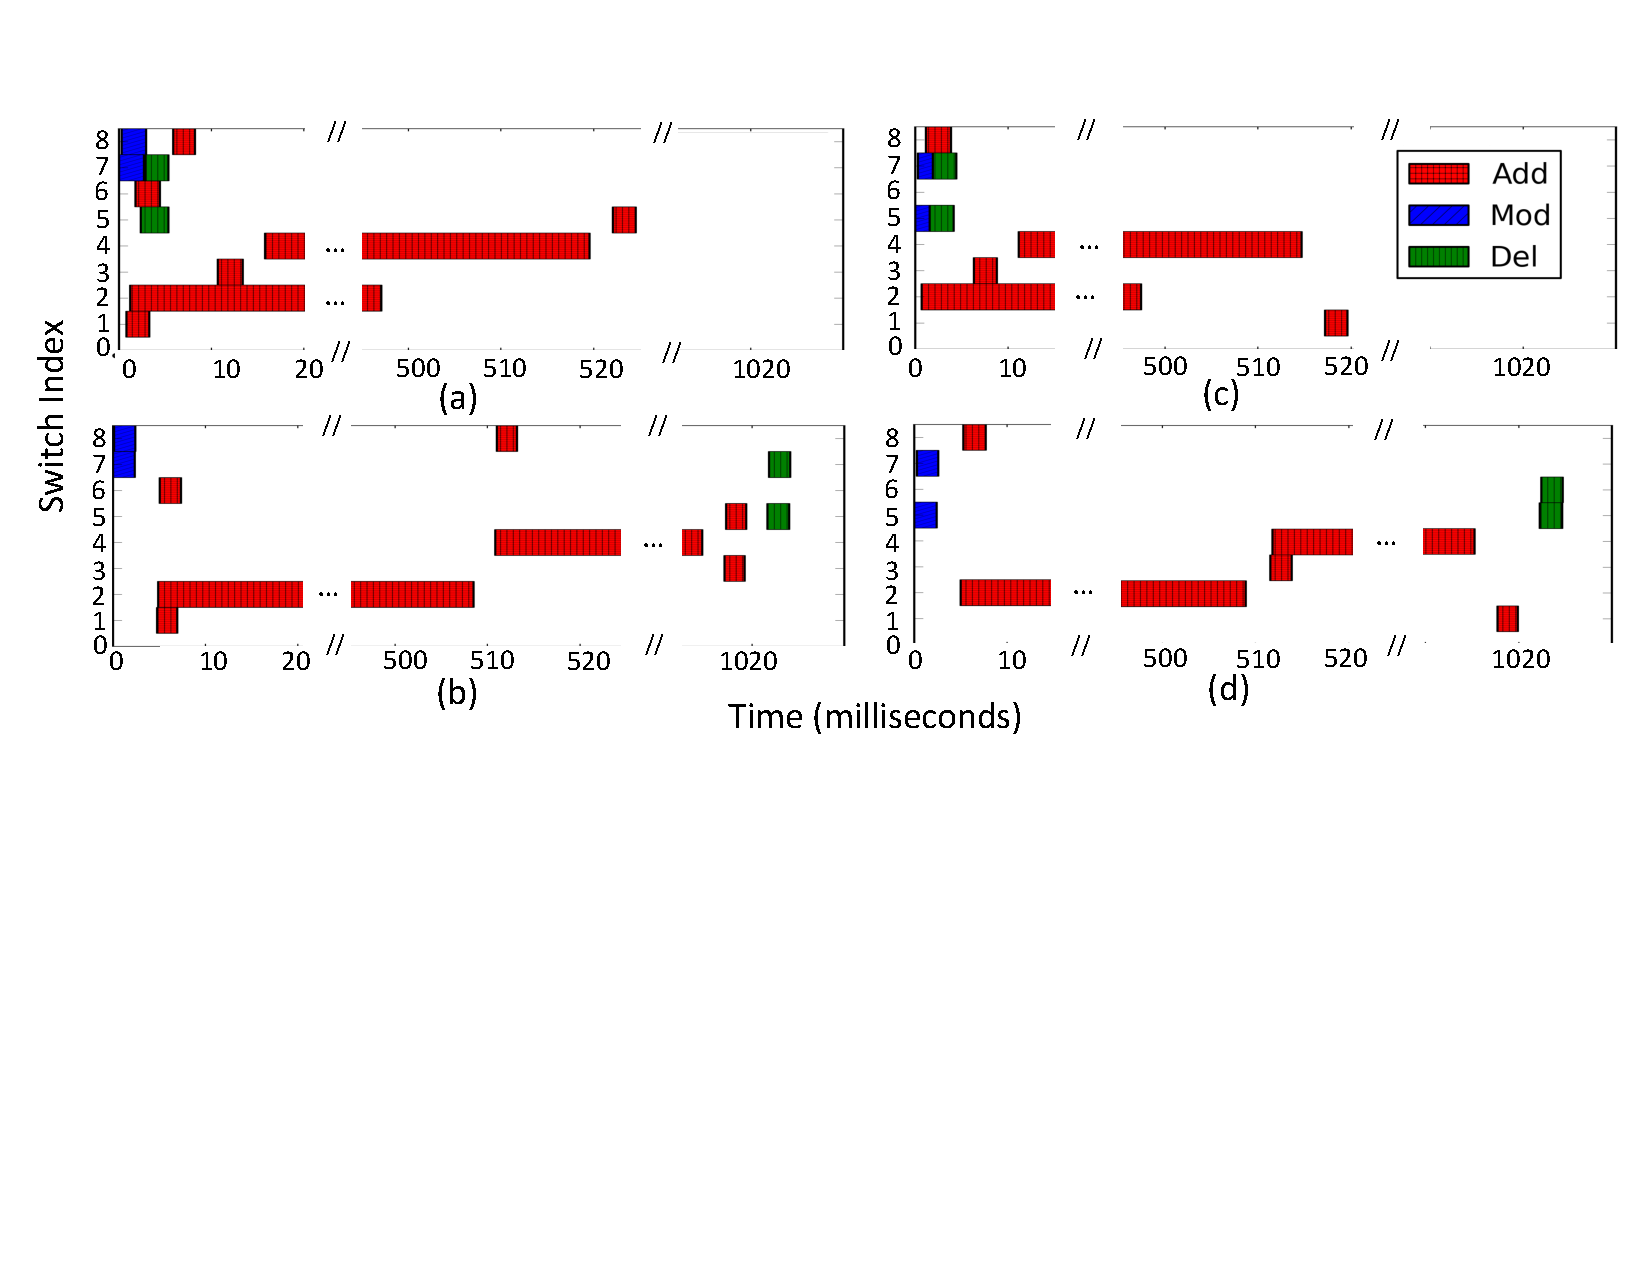
\includegraphics[width=0.8\textwidth]{figs/bandwidth}
        \end{minipage}
\end{figure*}
